\chapter{Thesis Contributions}
The general contribution of the thesis is a safety-critical design approach that employs formal methods at various stages of software development such as requirements specification and software design, and a power-efficient allocation of software to hardware while satisfying timing and reliability of the software in a distributed environment. It satisfies the research goals explained in Subsection~\ref{research_challenges} via the following contributions: a requirements specification language tailored to embedded systems~\cite{Mahmud2015ReSA:Systems}\cite{resatool}, formal analysis of the specifications~\cite{resatool}\cite{Mahmud2017SpecificationLogic} via formal and knowledge-based methods, formal analysis of large-scale Simulink models~\cite{Filipovikj2018SimppaalModels} and efficient mapping of software to hardware in the context of distributed architecture~\cite{Mahmud5222}\cite{Mahmud2019Power-awareOptimization} via integer-linear programming and metaheuristics. 

\section{Design Workflow: Contributions Overview}
Figure~\ref{fig_workflow} illustrates the workflow of an embedded software development that make of use our contributions. The workflow is contextualized in the automotive software development where Simulink, EAST-ADL and AUTOSAR architectural language are used. 
\begin{figure}[h]
	\centering
	\ifpdf
	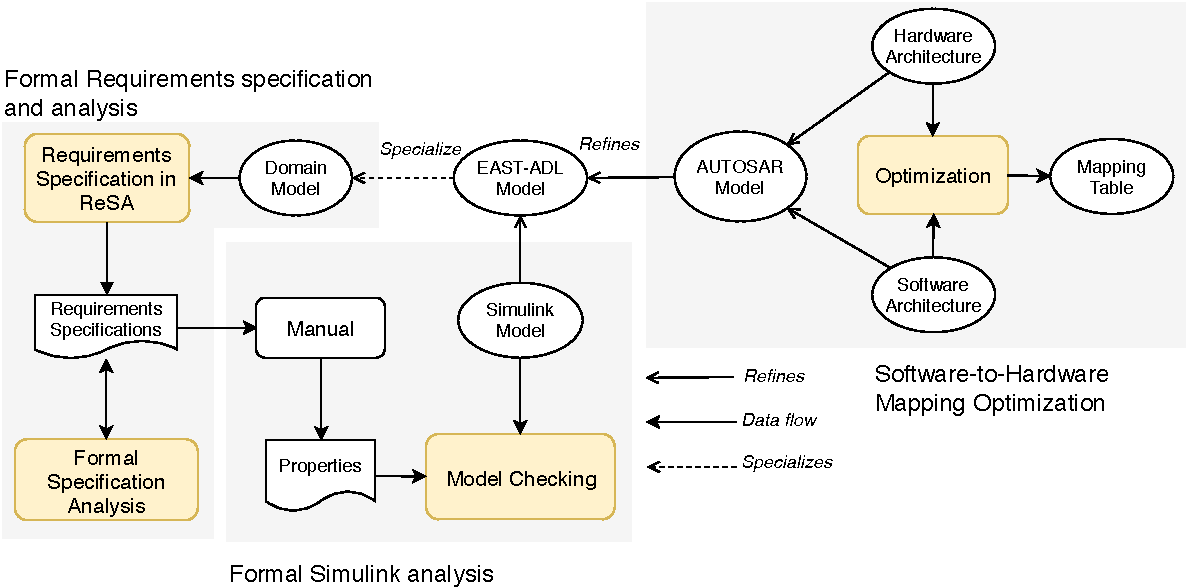
\includegraphics[width=\linewidth]{images/workflow}
	\else
	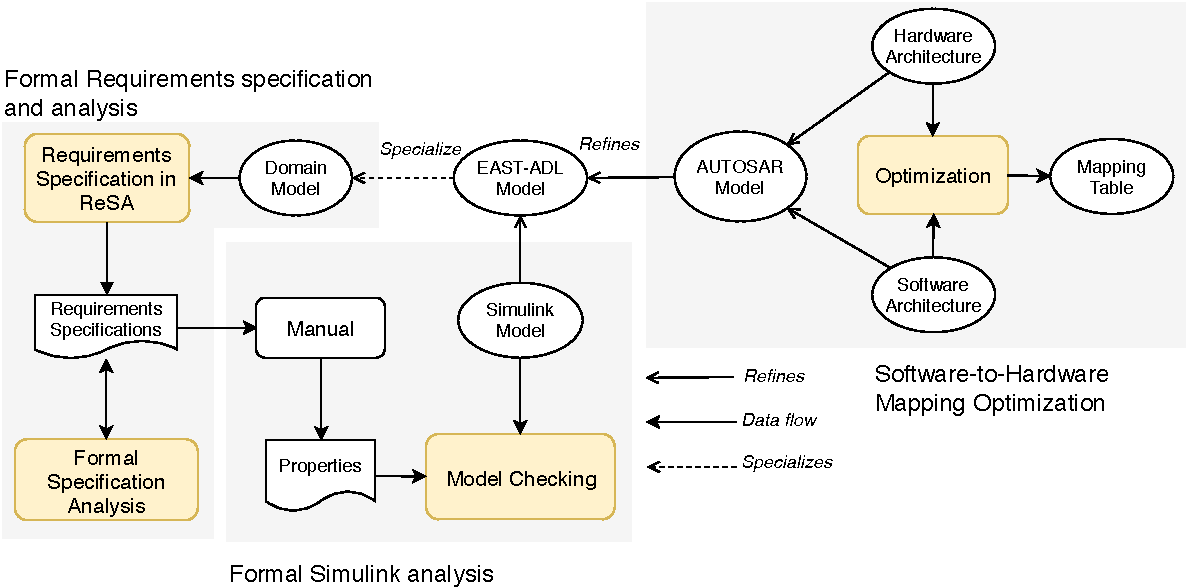
\includegraphics[width=.8\linewidth]{images/workflow.eps}
	\fi
	\caption{Thesis contributions workflow.} 
	\label{fig_workflow}
\end{figure}

Initially the textual requirements are specified in our domain-specific language ReSA, which is a constrained natural language tailored to embedded systems. The ReSA editor supports content completion as it is connected to a system model, which contains instantiation of words/phrases. If the ReSA editor is required to be domain-specific, e.g., to the automotive domain that employs EAST-ADL, the system model is specialized to the later model, thus enabling requirements specifications by accessing ESAST-ADL model elements from the editor. To check the consistency, the ReSA specifications are translated into Boolean and description logic, subsequently, analyzed via SAT solver and inference engine (or reasoner), respectively.

After the quality of the specifications are improved, i.e., become unambiguous,  comprehensible, consistent, they can be used in the verification of behavioral software designs. In this thesis, we consider the software design is made via Simulink, which is one of the most widely integerated environment for modeling, simulation and analysis of embedded system models. In order to rigorously analyze a Simulink model, we transform it automatically into a formal model, i.e., a network of stochastic timed automata. Subsequently, the latter is analyzed via statistical model checking against properties initially expressed in ReSA, but manually translated into the query (properties) language of the model checker, i.e., probabilistic weighed-metric temporal logic (PWMTL).

The Simulink model, at the architectural level, is represented by an EAST-ADL software architecture at the implementation level, i.e., via an AUTOSAR software architecture, which consists of software components that communicate through virtual function bus (VBS).  Note that, the refinement from the AUTOSAR model to the Simulink model is manual, which is the normal practice, however, the Simulink model composition (or structure) is automatically generated. The software architecture complements the Simiulink model with computational resource specifications, i.e., via runnables, which are schedulable piece of code (or objects) by the AUTOSAR OS. Moreover, it complements with other resource specifications, e.g., power specification, interface specification of the underlaying hardwares. In this regard, we propose (near) optimal software to hardware optimization techniques that incorporate the timing and reliability of software applications as constraints, and optimizes the power consumption of the software.

The thesis contributions are summarized as follows:
\section{Contr.~1: The ReSA Language}\label{rc_resa}
We propose a domain-specific and constrained natural language, both at the syntax and semantics level, which is designed to improve comprehensibility and reduce ambiguity of embedded systems requirement specifications. The language employs concepts from the embedded systems domain, e.g., \textit{System}, \textit{Parameter}, \textit{Device}, \textit{State}, \textit{Mode}, \textit{Entity}, to typeset domain-specific words/phrases. Besides grammatical rules (or syntax), semantic relations between the concepts limit on the possible construction of the specifications, e.g., grammatically the ``The ASL shall limit the driver.'' specification is correct, but semantically, it makes no sense. To solve this problem, the ReSA type system imposes on the a type constraint on the relation between instances ``The ASL''\textit{:system} and ``the driver''\textit{:user}.

\subsection*{Syntax}
The language design is modular, i.e., it uses sentence catagories, e.g., \textit{Simple}, \textit{Compound}, to structure the specifications, thus improve comprehensibility and reduce ambiguity. It also allow complex specifications by inductively applying the grammer rules of the language. The following context-free grammar is a snippet of the ReSA language. 
\begin{bnf*}
	\bnfprod{specification}
	{\bnfpn{simple} \bnfor \bnfpn{complex}\bnfor\bnfpn{nested-complex} ...}\\
	\bnfprod{simple}
	{\bnfpn{mainClause} .} \\%\bnftd
		\bnfprod{complex}
	{\bnfpn{subClause}, \bnfpn{mainClause}.} \\%\bnftd
	\bnfprod{mainClause}
	{\bnfpn{primitiveClause}\bnfor ...} \\%\bnftd
		\bnfprod{primitiveClause}
	{\bnfpn{sub} \bnfpn{verb} \bnfpn{obj}\bnfor...} \\%\bnftd
	\vdots
\end{bnf*}
{\footnotesize Note: please checkout the ReSA documentation for the complete grammar and its tool support from its webpage located at the URL {https://bitbucket.org/nasmdh/resa/src/master/}. }
\begin{example}[Adjustable Speed Limiter (ASL) Requirements]\label{ex_resa_example}
	ASL is a speed control system found in Volvo trucks. It controls the vehicle speed to not exceed a certain speed, which is set by the driver or legal authorities. It consists around 300 fuctional and extra-functional requirements. Just to demo the usage of the language, we specify only four of ASL equirements.
\begin{elaboration}{0.95}
	\small
		\begin{tabular}{lp{.9\textwidth}}
			R1 & ASL:system shall send "the driver"\textit{:user} notification:status every 200ms. \\
			R2 &\begin{tabular}[t]{@{}l@{}}if ``driver:user'' selects ``ASL speed control''\textit{:mode} and\\
				\hspace{0.5cm}(vehicle is in ``pre-running'' mode or
				vehicle is in ``running'' mode)\\ then\\
				\hspace{0.5cm}ASL:system shall be enabled within 200ms and\\
				\hspace{0.5cm}``ASL enabled''\textit{:status} shall be presented to ``the driver''\textit{:user} \\ endif\end{tabular} \\
			R3 & After ASL:system is enabled, if IncButton\textit{:inDevice} is pressed, ASL:system shall be activated.\\
			R4 &if driver selects ``ASL speed control''\textit{:mode}
			then 
			ASL\textit{:system} shall be disabled.
		\end{tabular}
\end{elaboration}
\end{example}

\subsection*{Tool Support and Validation on ASL}
The language is implemented in the Xtext framework\footnote{\url{Xtext: https://www.eclipse.org/Xtext/}}, which is an Eclibse-based integrated development environment for the development of domain-specific and general-purpose languages. The ReSA editor, which is shown in Figure~\ref{fig_resagui}, supports content completion, errors/warring messages and boilerplate management. The editor is integrated to EATOP, i.e., the editor can be trigged from within the IDE, moreover, the content-completion feature dispalys contents of the EAST-ADL model elements, hence enabling consistent use of vocabularies during specification. The ReSA tool as a standalone, and as a plugin for EATOP, can be downloaded from the URL {\small \url{https://bitbucket.org/dashboard/overview}}. 
\begin{figure}[h]
	\centering
	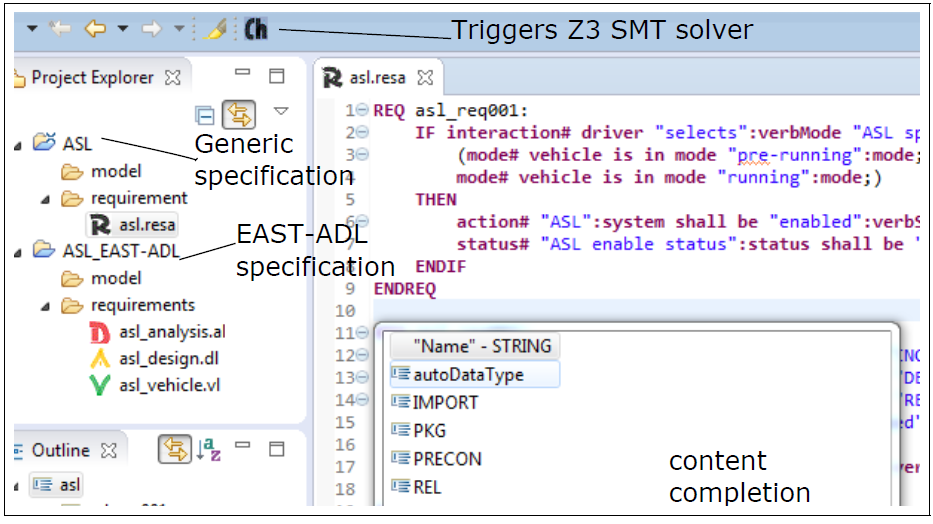
\includegraphics[width=0.7\linewidth]{images/resagui}
	\caption{The ReSA graphical user interface (GUI).}
	\label{fig_resagui}
\end{figure}

The language as well as its tool support is validated on the 300 ASL requirements, which are initially expressed in natural lanugage. The requirements distribution is as shown in Figure~\ref{fig_ASLreqs}, i.e., in terms of the types of requirments. The requirements are rewritten in ReSA, and Figure~\ref{fig_ASLreqsresult}shows the sentence catagories (or boilerplates) employed to specify the requirments. In general, the language is expressive,  though is constrained., and over a period of time, more and more constructs are added to improve the expressiveness.
 \begin{figure}[h] 
 	\centering
 	\subfloat[Types of ASL Requirements.\label{fig_ASLreqs}]{% 
 		\centering
 		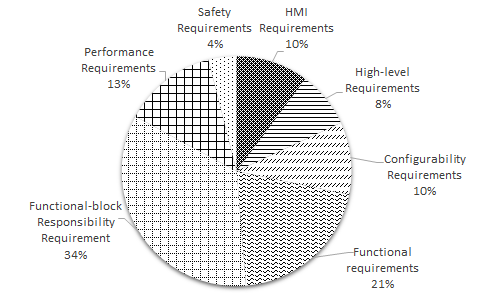
\includegraphics[width=0.45\textwidth]{images/aslreq}
 	} \hfill
 	\subfloat[Distribution of ASL boilerplate types.\label{fig_ASLreqsresult}]{% 
 		\centering
 		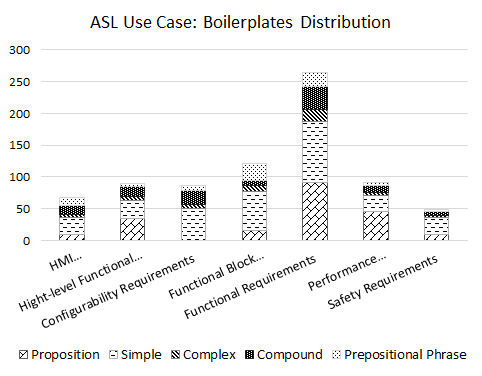
\includegraphics[width=0.45\textwidth]{images/aslbp} 
 	} 
 	\caption{Requirements specification ontology (screenshot from Prot\'eg\'e tool).} \label{fig_ontology}
 \end{figure}
\section{Contr.~2: {Formal Analysis of ReSA Specifications}}\label{rc_resaanalysis}
The editor shows syntax and typing warning and error messages. However, such static analysis are rudimentary since the analysis per specification. In this contribution, we propose two methods of consistency analysis: \textit{SAT-based} anaysis and \textit{ontology-based} analysis. 

\subsection*{SAT-based Analysis}
Boolean satisfiability (also known as SAT) can informally defined as the problem of finding truth-values (or assignments of boolean variables) such that a Boolean formula holds. It is NP-complete, however, there exist efficient heuristic algorithm which solve SAT problems of large-size, i.e., that consist of thousands of Boolean variables. Thus, first we transform the ReSA specifications into Boolean expressions~\cite{resatool}, then we formulate the problem of finding inconsistency the Boolean expressions in terms of SAT as follows:
\begin{definition}[Inconsistency of Specifications]
	Let $\Phi = \{\Phi_1, \Phi_2,\dots,\Phi_n\}$ is the ReSA specifications after translating ReSA specifications into Boolean expressions, where  $\Phi\in N$ is a Boolean formula and denotes a requirement specification. Thus, the set Boolean expressions $\Phi$ is inconsistent if the expression $\Phi_1 \land \Phi_2 \land\dots\land \Phi_n \Rightarrow false$ holds, that is, there exists at least one expression that cannot be satisfied, i.e., $\Phi_i\models false$.
\end{definition}
\begin{example}
Assume that we want to check the consistency of the requirements that are specified in Example~\ref{ex_resa_example}. Figure~\ref{fig_z3} shows the translation of the specifications into Boolean expressions (i.e. in Z3  SMT-LIB format). Each expression is asserted before the Z3 solver is called using the command $(check-sat)$. Some clauses are resolved for negation and opposite words, e.g., the fact that ``enabled'' is opposite of ``disabled'' implies $p_5=p_7\neq p_{11}$. The solver returned ``unsat (R2 R4 R1\_Assertion)'',  which means, the expressions are inconsistent and indicates the specifications that are responsible for the inconsistency (or unsat-core).
\end{example}
\begin{figure}[h]
	\centering
	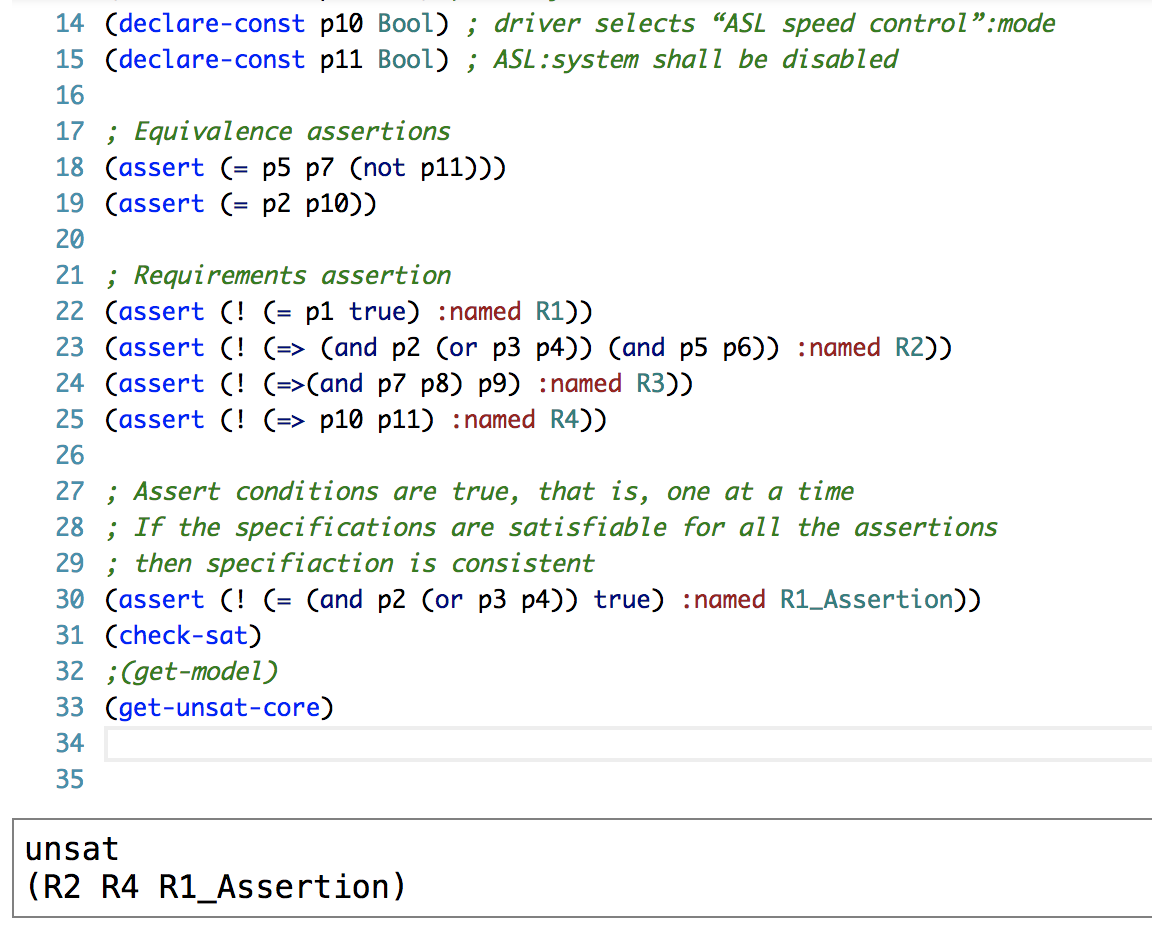
\includegraphics[width=0.7\linewidth]{images/z3}
	\caption{The ReSA specifications R1- R4 encoded as Z3 format, and the unsat-core feedback from the Z3 solver, to localize source of the inconsistency.}
	\label{fig_z3}
\end{figure}

The SAT-based analysis, although, easy and scalable, it does not allow rigorously analysis. This is due to the fact that the Boolean (or propositional) variables abstract away details of the clauses in the specifications. The ontology-based approach solves this problem with trade off over scalability.

\subsection*{Ontology-based Analysis}
Ontology as a knowledge representation technique can be used to capture the intricate relations of words/phrases of specifications, e.g., synonyms, antonyms, generalization. Morover, it can be used to capture the syntax of the specifications as well, essentially modeling the the ReSA specification as a concrete requirements specification ontology. 

Besides the challenge of constructing the ontology, accurate representation of the specifiactions is crucial to a certain degree for the ontology to be useful, i.e., the specifications should be interpreted linguistically. In this research, we propose the \textit{event-based} semantics approach~\cite{Mahmud2017SpecificationLogic} to construct the meaning of each specification compositionally fromts its constituents (or grammar units). The event-based semantics, which is based on the first-order logic, uses an existentially quantified events to relate words/phrases (or arguments of predicate) , clauses, adjuncts of a sentence~\cite{Mahmud2017SpecificationLogic}, e.g., the clause ``ASL:system shall limit ``vehicle speed'':parameter'' is represented as $\exists e$[limiting($e$) \& Agent(ASL) \& Recipient(vehicle speed)], where Agent and Recipient are known as \textit{thematic} roles, which define the semantic roles of the arguments in the clause.  Since the requirement specifications entail technical words/phrase, the thematic roles of these arguments are not obvious, so we extended the thematic roles into the ReSA concepts, e.g., any instance of \textit{System} or \textit{User} is \textit{Agent}, similarly instances of \textit{Parameter} is \textit{Recipient}. In this way, the interpretation of the clauses become domain-specific.

Following the event-based semantics, the ReSA specifications are translated into description logic as ontology. Once the ontology is constructed considering the event-based semantic, thematic roles, lexical relation, we check the consistency of it via an inference engine (or reasoner), which is a software program that applies logical rules on a logical system, such as the ontology, to obtain new information.
\begin{definition}[Inconsistency of Specifications]
	The requirements specification ontology is inconsistent if there does not exists an interpretation (or a model) $M$ that satisfies the terminological assertions $T$ and the concrete assertions $A$, that is, $M \not\models ax$, where: $ax \in T \cup A$, and $T$ is a set of terminological assertions and $A$  a set of facts (or concrete assertions).
\end{definition}
%\begin{figure}
%	\centering
%	\subfloat[Concepts.\label{fig_continuous}]{% 
%		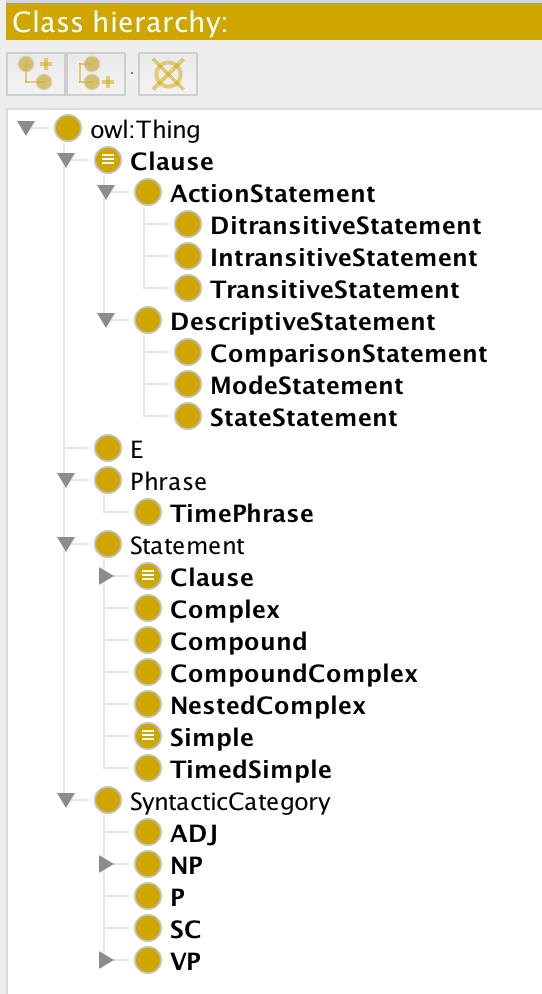
\includegraphics[width=0.3\textwidth]{images/ro_concepts}
%	} \hfill
%	\subfloat[Object properties.\label{fig_discrete}]{% 
%		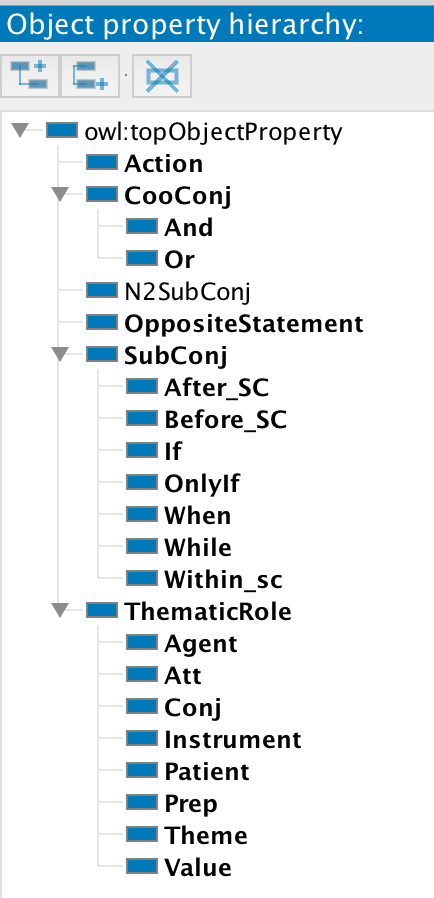
\includegraphics[width=0.3\textwidth]{images/ro_objects} 
%	} 
%\hfill
%\subfloat[Individuals.\label{fig_discrete}]{% 
%	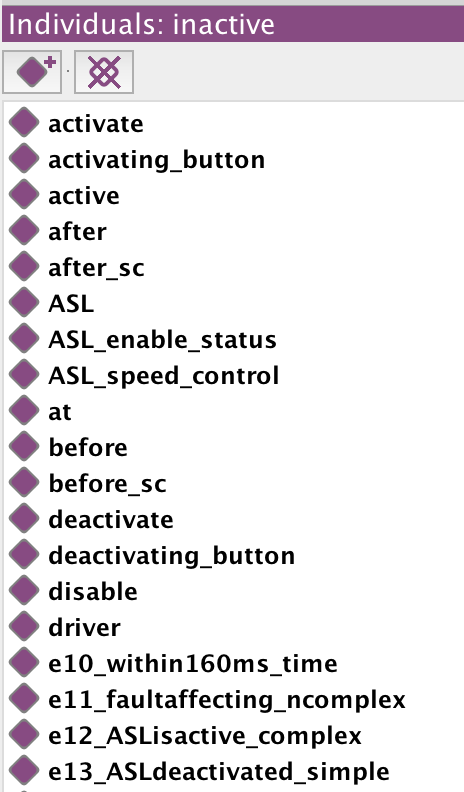
\includegraphics[width=0.3\textwidth]{images/ro_individuals} 
%} 
%	\caption{Requirements specification ontology (screenshot from Prot\'eg\'e tool).} \label{fig_ontology}
%\end{figure}

\section{Contr.~3: {Scalable Formal Analysis of Simulink Models}}\label{rc_sim}
Several research exist on formal anlaysis of Simulink models, e.g., using theorem proving, exact model checking, statistical model checking. Many of the proposed solutions are  limited either due to frequent user involvement or scalability issues. In this thesis, we propse a scalable formal analysis of larege-scale Simulink models via statistical model checking. The Simulink models can be discrete, continuous or hybrid, moreover, they can consist of atomic and composite Simulink blocks that are scattered on multiple files, which is a practical scenario. Essentially, we consider typical industrial Simulink models, e.g., the brake-by-wire and adjustable speed limiter Simulink models from VGTT~\cite{Filipovikj2018SimppaalModels}.

Our approach has the following important characterstics: (i) the transformation employs continous and discrete transformation patterns, which are generic and reusable, thus can be applied to any Simulink blocks; (ii) the transformation preserves the execution orders of the Simulink blocks; (iii) it is robust, i.e., it handles various models such as continuos, discrete, hybrid, and models which contain blocks that execute with different sampling rates, also known as multi-rate.

\subsection*{Transformation Patterns} 
The continuous-time and discrete-time stochastic timed automata (STA), which are shown in Figure~\ref{fig_patterns}, are used to transform the continuous-time and discrete-time Simulink blocks into their respective STAs. The automata in both cases makes transition from the ``Start'' location to the ``Operate'' location at the global time $sn*IAT$, which is determined according to each block's order of execution $sn$, i.e., the lower $sn$, the sooner the automaton makes  transition to the ``Operate'' location, and $IAT$ is an infinitesimal inter-arrival time between the release of the automata. In the case of the continuous-time STA pattern, the automaton makes a loop transition at the ``Operate'' location every infinitesimal sample time, which is distributed exponentially according to the rate  $\lambda=1000$. Whereas in the case of discrete-time STA pattern, it makes a loop transition every $ts$ sample time with probability of 1, as there is only one edge that goes out of the location and the delay transition is distributed uniformly in the interval $[ts,ts]$.
\begin{figure}[h] 
	\centering
	\subfloat[Continuous-time.\label{fig_continuous}]{% 
		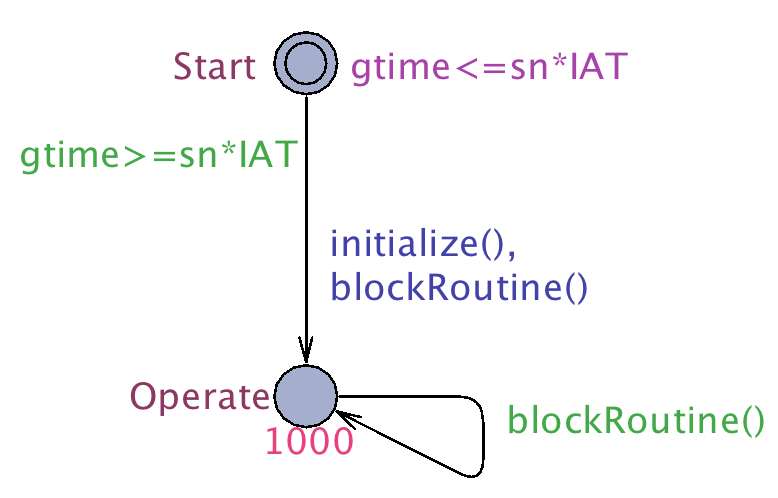
\includegraphics[width=0.45\textwidth]{images/continuous-sta}
	} ~
	\subfloat[Discrete-time.\label{fig_discrete}]{% 
		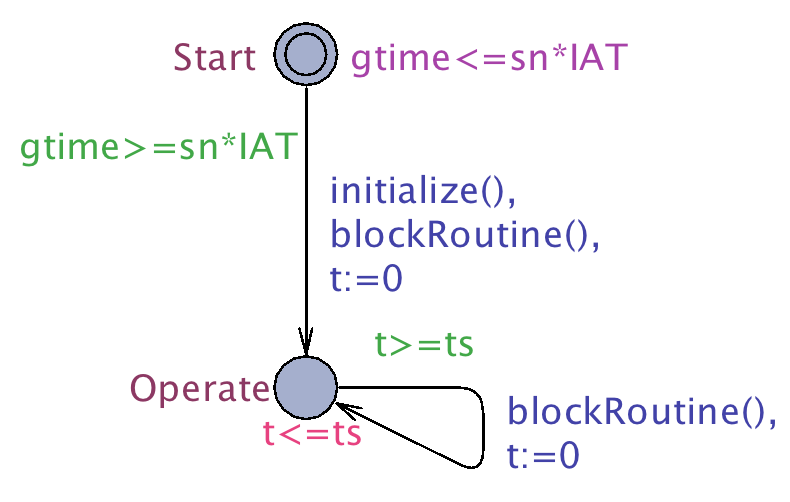
\includegraphics[width=0.45\textwidth]{images/discrete-sta}
	} 
	\caption{STA transformation patterns.} 
	\label{fig_patterns}
\end{figure}

\subsection*{Simulink to NSTA Transformation Process} 
Besides proposing the transformation patterns, we provide an automatic transformation of a Simulink model to its equivalent network of STA by applying the following tasks:
\begin{enumerate*}[label=(\roman*)]
	\item the Simulink model is simulated, subsequently, the sorted-order list, which contains the execution order of the Simulink blocks, is extracted.
	\item in case the model is hierarchical, the execution order is flattened first, thus generating a flattened sorted-order list;
	\item the Simulink model is parsed, as a result, each block is translated into a stochastic timed automata via the corresponding transformation pattern. The sorted-order number $sn$ is instantiated from the sorted-order list on the fly.
	\item any non-computational blocks is accounted in the transformation but are not trasformed into automata, e.g., the Mux, SubSystem blocks;
	\item the connections between the blocks are translated into global variables, which acts as communication between the automata.
\end{enumerate*}
Please checkout Section~3 of~\cite{Filipovikj2018SimppaalModels} for the detailed discussion on the transformation as well as its soundness proof.

%\begin{figure}
%	\centering
%	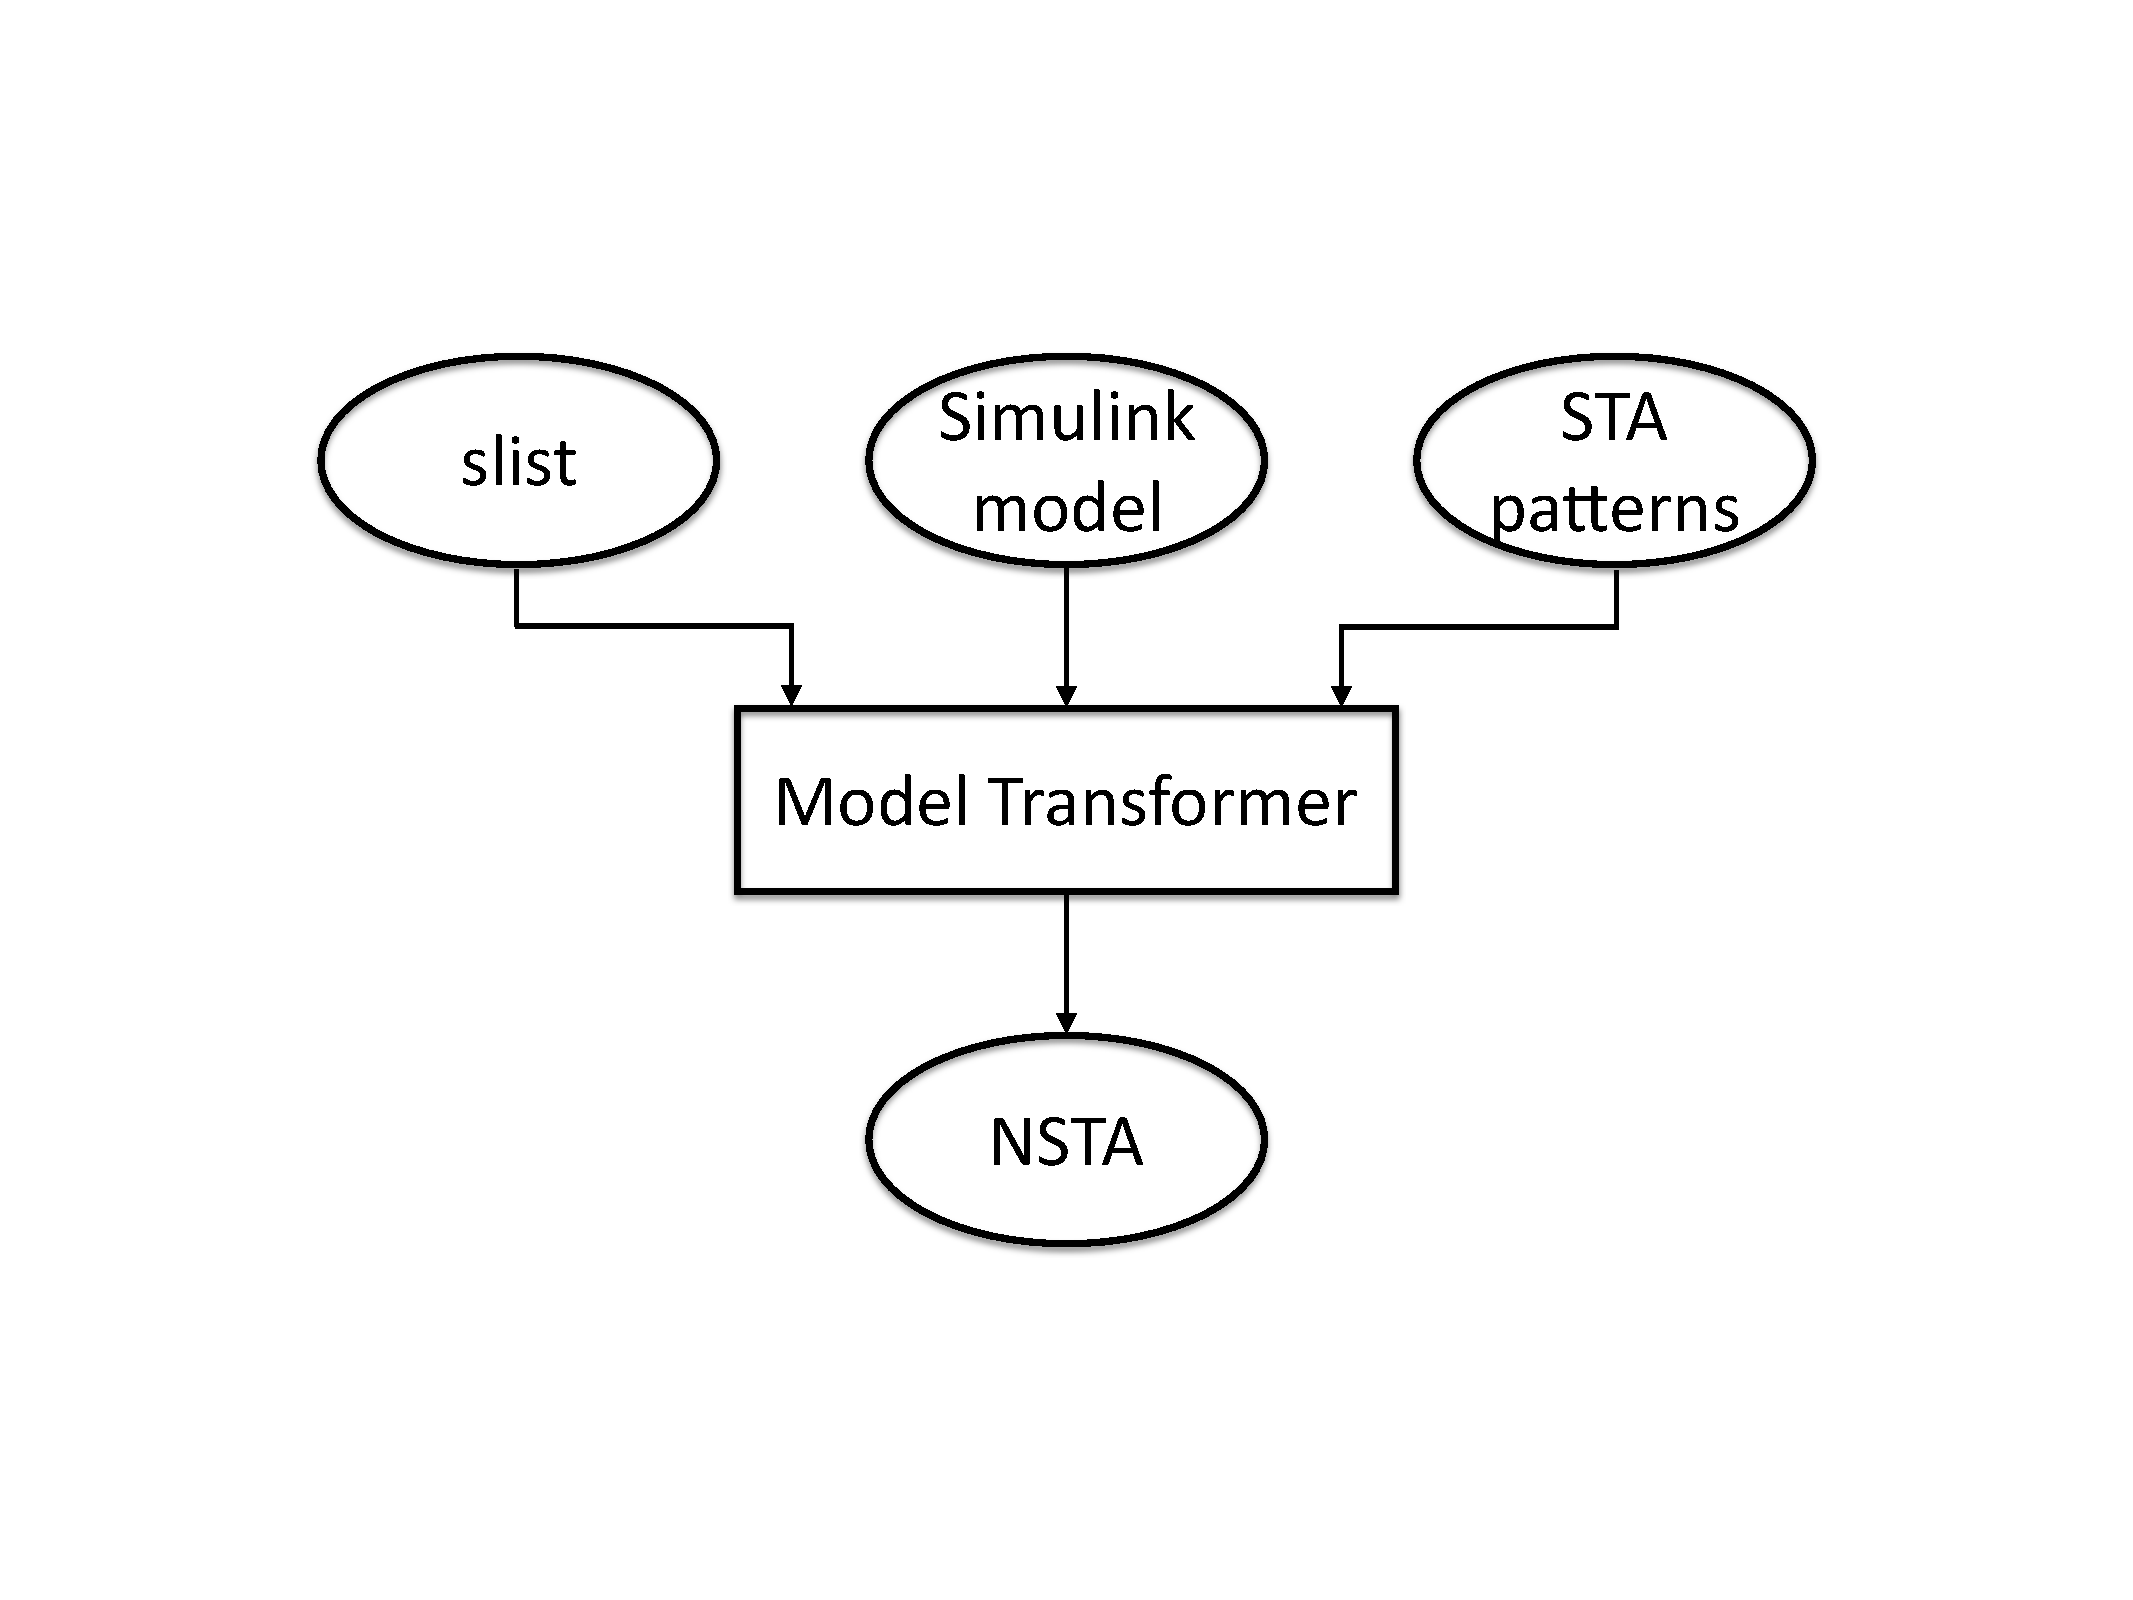
\includegraphics[width=0.6\linewidth]{images/simulinkapproach}
%	\caption{Simulink to NSTA Transformation}
%	\label{fig_approachworkflow}
%\end{figure}

\subsection*{Validation on the Brake-by-wire Use Case} 
Our approach is applied on an industrial brake-by-wire Simulink model, which is a prototype developed for academic use by VGTT. The model consists of 320 blocks, of which 19 are discrete blocks, 26 constant blocks and the rest are continuous-blocks. The model design consists of of modules that collects sensory data, e.g., vehicle speed, pedal position, and computes the proportional torque force that is applied on the wheels to brake the vehicle. Besides, it has the  anti-braking functionality (i.e., the ABS) to avoid (or minimize) skidding, which occurs when the slip rate of a wheel is greater than its friction coefficient. 

The BBW requirements are initially specified in ReSA, subsequently are translated into PWMTL properties manually by using monitors (or observers), which are stopwatch stochastic priced timed automata. The monitors are modeled for particular requirements, and basically observe the progressionf the execution of the automata.
\begin{example}[Statistical model checking of BBW]\label{ex_resa}
	The BBW model is automatically transformed into a network of STAs, and we modeled the monitor (Appendix A) to represent 5 functional and timing requirements, of which 3 requirements are shown in the box below for illustration. \vspace{0.2cm}
\begin{elaboration}{0.9}
	\small
	{}
	\begin{tabular}{lp{.85\textwidth}}
	R1 & The brake request shall be computed within 10 ms. \\
	R3 & The brake request shall be be propagated to two different wheel actuators within 4 ms.\\
	R4 & If the brake request is 0, then the ABS shall set the torque to 0. \\
\end{tabular}
\end{elaboration}
\end{example}

Figure~\ref{fig_smcresult} shows the PWMTL propeties and their model checking results. R1 and R3 are safety requirements which are expressed using the $\Box$ operator as indicated by R1$_{BBW}$ and R3$_{BBW}$ PWMTL properties, respectively. R4 is a conditional requirement which is expressed using the $\Diamond$ operator as indicated by R4$_{BBW}$ PWMTL property. Each result shows the probability interval of satisfying the property (if qualitative) or the probability of satisfying a property (if quantitatiy), confidence level, the number of runs and the time needed by the model checker to return the result. For all properties, the probability interval (or confidence interval) approximates $[0.99,1]$ with confidence level $\approx0.999$, which can be interpreted as ``the properties are satisfied`` if the probability requirements lower-bound are in the degree of 0.99. However, in many safety-critical applications, the requirement on the probability is normally high, e.g., 0.999999 (essentially approximates to ``no failure should happen''). In this case, the interval should be more precise, which can be achieved by lowering $\alpha$ and $\beta$ of the hypothesis testing, which are the probabiliy of accepting false positive (i.e., accepting H$_0$ when H$_1$ holds) and false negative (i.e., accepting $H_1$ when $H_0$ holds), respectively~\cite{David2011StatisticalAutomata}.
\begin{figure}[h]
	\centering
	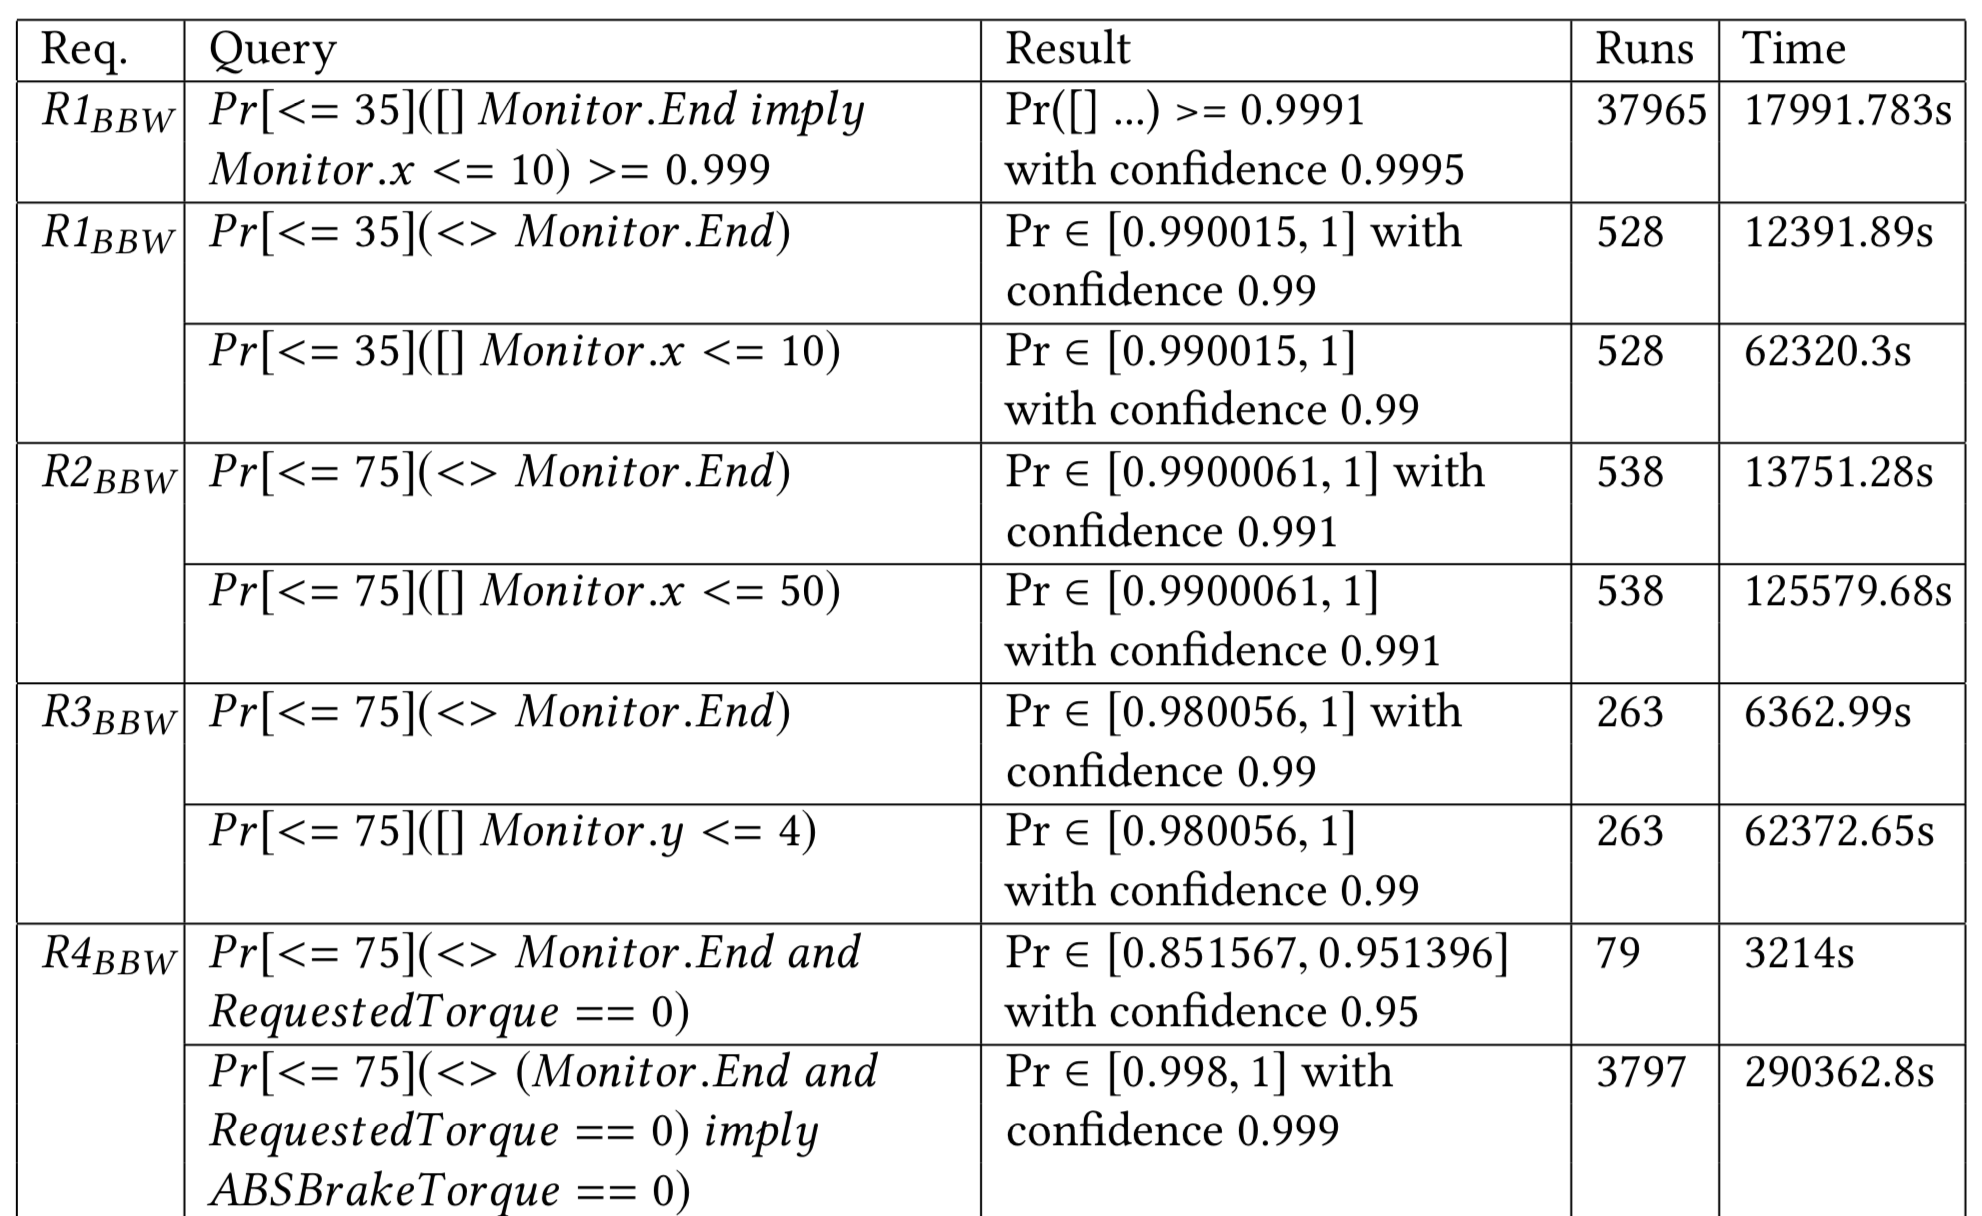
\includegraphics[width=0.8\linewidth]{images/smc_result}
	\caption{BBW SMC result snippet from UPPAAL SMC.}
	\label{fig_smcresult}
\end{figure}

\section{Contr.~4: ILP-based Software Allocation}\label{rc_ilp}
Safety-critical systems are usually resource constrained, that is, the execution hardware platform has limited computational resources and power/energy sources. Therefore, the system should be designed efficiently especially critical system resources such as power in order to accommodate complex safety-critical software functionality. In this section, we propose exact method of mapping software to hardware in order to optimize the total power consumption of a distributed safety-critical software via ILP, which is needed when highly-efficient design is needed especially small-scale sofware applications, e.g., software components not exceeding 10.

\subsection*{System Model}
We consider an AUTOSAR distributed safety-critical software that can be mapped to multiple computing nodes (or units), which are heterogeneous computing systems with respect to power specification, failure rate and processing speed. The software has end-to-end timing and reliability requirements, therefore, the mapping must satisfy the requirements. In order to meet the reliability requirement, the mapping applies fault tolerance by replicating software components subsequently mapping the replicas on different computing units. Moreover, the task and messages that realize the safety-critical software functionality are scheduled using a fixed-priority preemptive scheduling policy and fixed-priority non-preemptive scheduling policy (over a  CAN bus), respectively.

The AUTOSAR software functionality is implemented by Runnables that communicate over the virtual function bus (VFB), which abstracts the details of the run-time environment. We assume the runnables are triggered periodically and have multiple worst-case execution times as they can executed on processors that have different processing speed.
\begin{figure}[h]
	\centering
	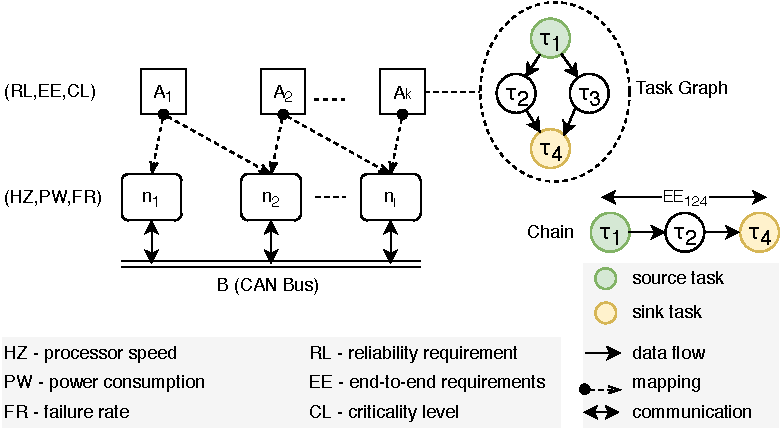
\includegraphics[width=0.8\linewidth]{images/system_model.pdf}
	\caption{Computation time of the various algorithms for solving different instances of the software allocation problem.}
	\label{fig_allocationtime_ilp_metaheuristic}\vspace{-0.4cm}
\end{figure}

\subsection*{ILP Model}
Consider that the mapping solution is represented by a vector of binary matrices $\textbf{x}=\{\textbf{x}_1:1,...,K\}$, where \ttxkij represents the mapping of the software component $\sss{q}[k][ij]$ to the computing node $\ssb{n}[j]\in \mathcal{N}$. 
\begin{equation}
\label{eqn_solution}
\bspx{k}=
\begin{bmatrix} 
\ssx{k}{11} & \ssx{k}{12} & \dots & \ssx{k}{1K}\\
\ssx{k}{21} & \ssx{k}{22} & \dots & \ssx{k}{2K}\\
\vdots & \vdots & \ddots & \vdots\\
\ssx{k}{N1} & \ssx{k}{N2} & \cdots & \ssx{k}{NK}
\end{bmatrix}
\end{equation}
The power consumption of a software application $\{c_i:i=1,...,n_C\}$ that is mapped to computing units $N'\in N$ is calculated as the sum of the power consumption of each node $n_h\in N'$, thus $\mathcal{P}_{total}(x)=\sum_{n\in N'}{\mathcal{P}(u_n(x))}$, where $\mathcal{P}(u)$ is the power consumption of a computing node which linearly proportional to its utilization~\cite{Mahmud5222}. The utilization of a computing node is the sum of the utilization of its constituent tasks that realize corresponding software components.
\begin{align}
	(u_1,...,u_K)(\x)=\sum_{k=1}^{K}\sum_{\tau\in T_{c_i}}{\xkij*\frac{WCET_\tau}{P_\tau}},
\end{align}
where $T_{c_i}$ is the set of tasks realizing the software component $c_i$, $WCET_\tau$ and $P_\tau$ are the worst-case execution time and  period of the task $\tau$.

\subsubsection{Tasks Deadline Constraint}
The mapping solution must satisfy the timing and reliability requirements imposed on the safety-critiacal application. We assume the taskset in each computing node is scheduled using a fixed-priority preemptive scheduler~\cite{Sha2004RealPerspective} and we check the schedulability via the classical worst-case response time analysis~\cite{Baruah2011Response-timeSystems}. Since the time analysis model involves recursion which is difficult to model as a linear model. Therefore, we construct linear logical constraints $\xi$ that corresponds to the valid tasksets that can potentially partitioned to computing nodes, and these tasksets are schedulable.

The logical system is constructed as follows: first we identify the possible partitions of the software components, $P=2^C$, then we check the schedulability of each partition and catagorize them per node, i.e., $Y_j=\{p\in P| isSched(p,n_j)\}$, where $sched$ is a boolean function that returns true if $p$ is schedulable on $n_j$.  A partition is identified by a sequence of 0s and 1s based on its costituent components, e.g., the id of the partition $\{c_1,c_4,c_5\}\subseteq \{c_1,c_2,c_3,c_4,c_5\}$ is $10011=19$. So, given the mapping $\x$, the partition id that is mapped to the computing node $n_j$ can be computed as
\begin{align}
	g_j(\x)=\sum_{i=1}^{N}{10^{N-i}\max_{1\leq k< K}\xkij}
\end{align}
where the $\max_{1\leq k< K}$ function returns 1 if at least one component replica is mapped $n_j$, otherwise returns 0, indicating no replica is mapped to that node. Thus, each node must have a valid partition that is schedulable as indicated in the logical constraint,
\begin{align}
\bigvee\limits_{p\in Y_j}g_j (\x)= id(p) ,
\end{align}
where $id(p)$ is a predicate that returns the id of the partition $p$.

\subsubsection{End-to-end Timing Constraint}
The age delay of a chain is computed according to the semantics discussed in~\cite{Feiertag2009ASemantics}\cite{mubeen2013support}. The response-time logical assertions ensure that every task in the distributed system are schedulable for a mapping \ttx. Therefore, we can safely check if the age delay of each chain satisfy its end-to-end timing requirement without the need to check the chain's constituent tasks are schedulable or not. Similar to the previous approach, we construct logical constraints $\eta$ that correspond to the valid set of mappings of chains on the network of computing nodes.  Given $\Gamma =\{\Gamma_i:i=1,...,N\}$ of chains, the set of possible mappings of each chain $\Gamma_i$ on a set of $\mathcal{N}^\Gamma$. Thus the set of valid mappings of each chain satisfy the end-to-end timing requirement is $Z_i=\{\gamma\in \mathcal{N}^\Gamma| ageDelay(\gamma) < EE_\gamma$.

\subsubsection{Software Application Reliability Constraint}
The reliability constraint refers to the probability that the application functions by the time $t$, i.e $[0,t]$~\cite{Goel1985SoftwareApplicability}. We assume that the reliability requirement of a software application is 0.99999999 over a 2-year operation time, which is to say  that the safety-critical system almost should not fail within the stated period. Furthermore, we assume that the mean-time to failure of the computing nodes is given as $10^6$ hours (0.0000001 per hour), which is the usual practice in many functional safety design.

Unless the the software application is replicated on one or more computing nodes, the reliability requirement is usually unattainable. So, the allocation strategy is basically to replicate sufficient software components to meet the requirement at the same time it should not exceed the limit so that the application consumes less power. However, the reliability calculation is not trivial as the replication results in functional inter-dependency of the computing nodes, in this case,  the series-parallel method does not apply. For this reason, we propose an exact method based on state enumeration~\cite{ExactMethodstoComputeNetworkRe- liability}, which basically enumerates all the possible configurations of the nodes  $PS$. Subsequently, the reliability of the application becomes the total probability of the configurations that enable the functioning of the application~\cite{Mahmud5222}.
\begin{definition}[Software Application Failure]
	A software application fails in the configuration $s\in\xi$ if there exists a component type $c_i$ where all of its replicas $Q_i$ \textit{fail}, otherwise, it functions, as shown in Equation (\ref{eqn_appreliability_milp_components}).  The component replica $q_i,j\in Q_i$ of type $c_i$ fails if $n_h$ fails, that is $s_h=0$.
\end{definition}
\begin{align}
f_s(x) = \floor[\Bigg]{\frac{\sum_if_{c_i}(x,s)}{N}}=
\begin{cases}
1 & \mbox{if } application \mbox{ functions}\\
0 & \mbox{if } application \mbox{ fails}
\end{cases}\label{eqn_appreliability_milp_components}
\end{align}

Thus, the reliability of the software allocation is
\begin{align}
\label{eqn_appreliability_milp}
Reliability(\x)=\sum_{s\in PS}f_s(\x)*p_s,
\end{align}
where $p_s$ is the probability that the computing nodes attain a configuration $s$ which is computed as $p_s=\prod_{m\in M}\big[(z_m*\lambda_m) + (1-z_m)*(1-\lambda_m)\big]$, where $z_m\in\{0,1\}$ indicates if the node fails (i.e., 0) or functions (i.e., 1), $\lambda_m$ is the failure rate of the node $m$ and $1-\lambda_m$ is the opposite of failure rate, i.e., that is the rate that it does not fail.
\subsubsection{ILP Problem}
The goal of the ILP optimization is to minimize the total power consumption, which is the objective function, and the constraints Equation (\ref{lbl_deadline_constraint}), (\ref{lbl_e2e_constraint}) and (\ref{lbl_reliability_constraint})ensure that the optimization satisfies the tasks deadline, end-to-end timing and reliability constraints, respectively.
\begin{align}
\label{eqn_const_func}
\min_{\x\in X} \mathcal{P}_{total}(\x) && \text{ Subjected to:}\\
\label{lbl_deadline_constraint} 
\bigvee\limits_{p\in Y_j} g_j (\x) &= id(p)& \mbox{ for all } j=1,..,|\mathcal{N}|\\ 
\label{lbl_e2e_constraint}
\bigvee\limits_{\gamma\in Z_j} h_j (\x) &= id(\gamma) & \mbox{ for all } j=1,..,|\Gamma|\\ 
\label{lbl_reliability_constraint}
\sum_{s\in PS}f_s(\x)*p_s &\leq \RL&,
\end{align}

\subsection*{Tool Support and Validation on Automotive Benchmark}
Our proposed ILP approach is validated on different size of software applications, i.e., applications with variable number of software components, cause-effect chains and degree of replication. The applications are synthesized according to the automotive benchmark proposed by Kramer et al.~\cite{Kramer2015RealFree}, which discusses a typical complexity of an AUTOSAR engine management system in terms of, e.g., the number and execution time of runnables, and the number and activation patterns of cause-effect chains. 

We prepared 6 software applications and an execution platform that consists 8 nodes. The smallest application consist of 4 components and the largest 10 components. Furthermore, the cause-effect chains varies from 10 to 60 and activation patters ranges from 2 to 4. Figure~\ref{fig_ilp_results} shows the result of the optimization from the CPLEX solver, that is, the power consumption and the computation time, respectively. In general, the optimization maps components to nodes with lower power specification and higher processor speed, however, this is not always the case since the end-to-end timing and reliability constraints can dictate the selection of different nodes, which consume more power as a result. Figure~\ref{fig_computationtime_ilp} shows a slow increase of computation time from until the application with 8 number of components, which took  6.06 sec, and rapidly increased to 30.3 sec and 129.4 sec allocating application with 9 and 10 components, respectively. The optimization took extremely large amount of time for applications that consist of more than 10 components, and more than 15 component the waiting time was intractable, thus the optimization was interrupted manually. 
\begin{figure}[h] 
	\centering
	\subfloat[Power consumption of nodes.\label{fig_powerconsumption_ilp}]{% 
		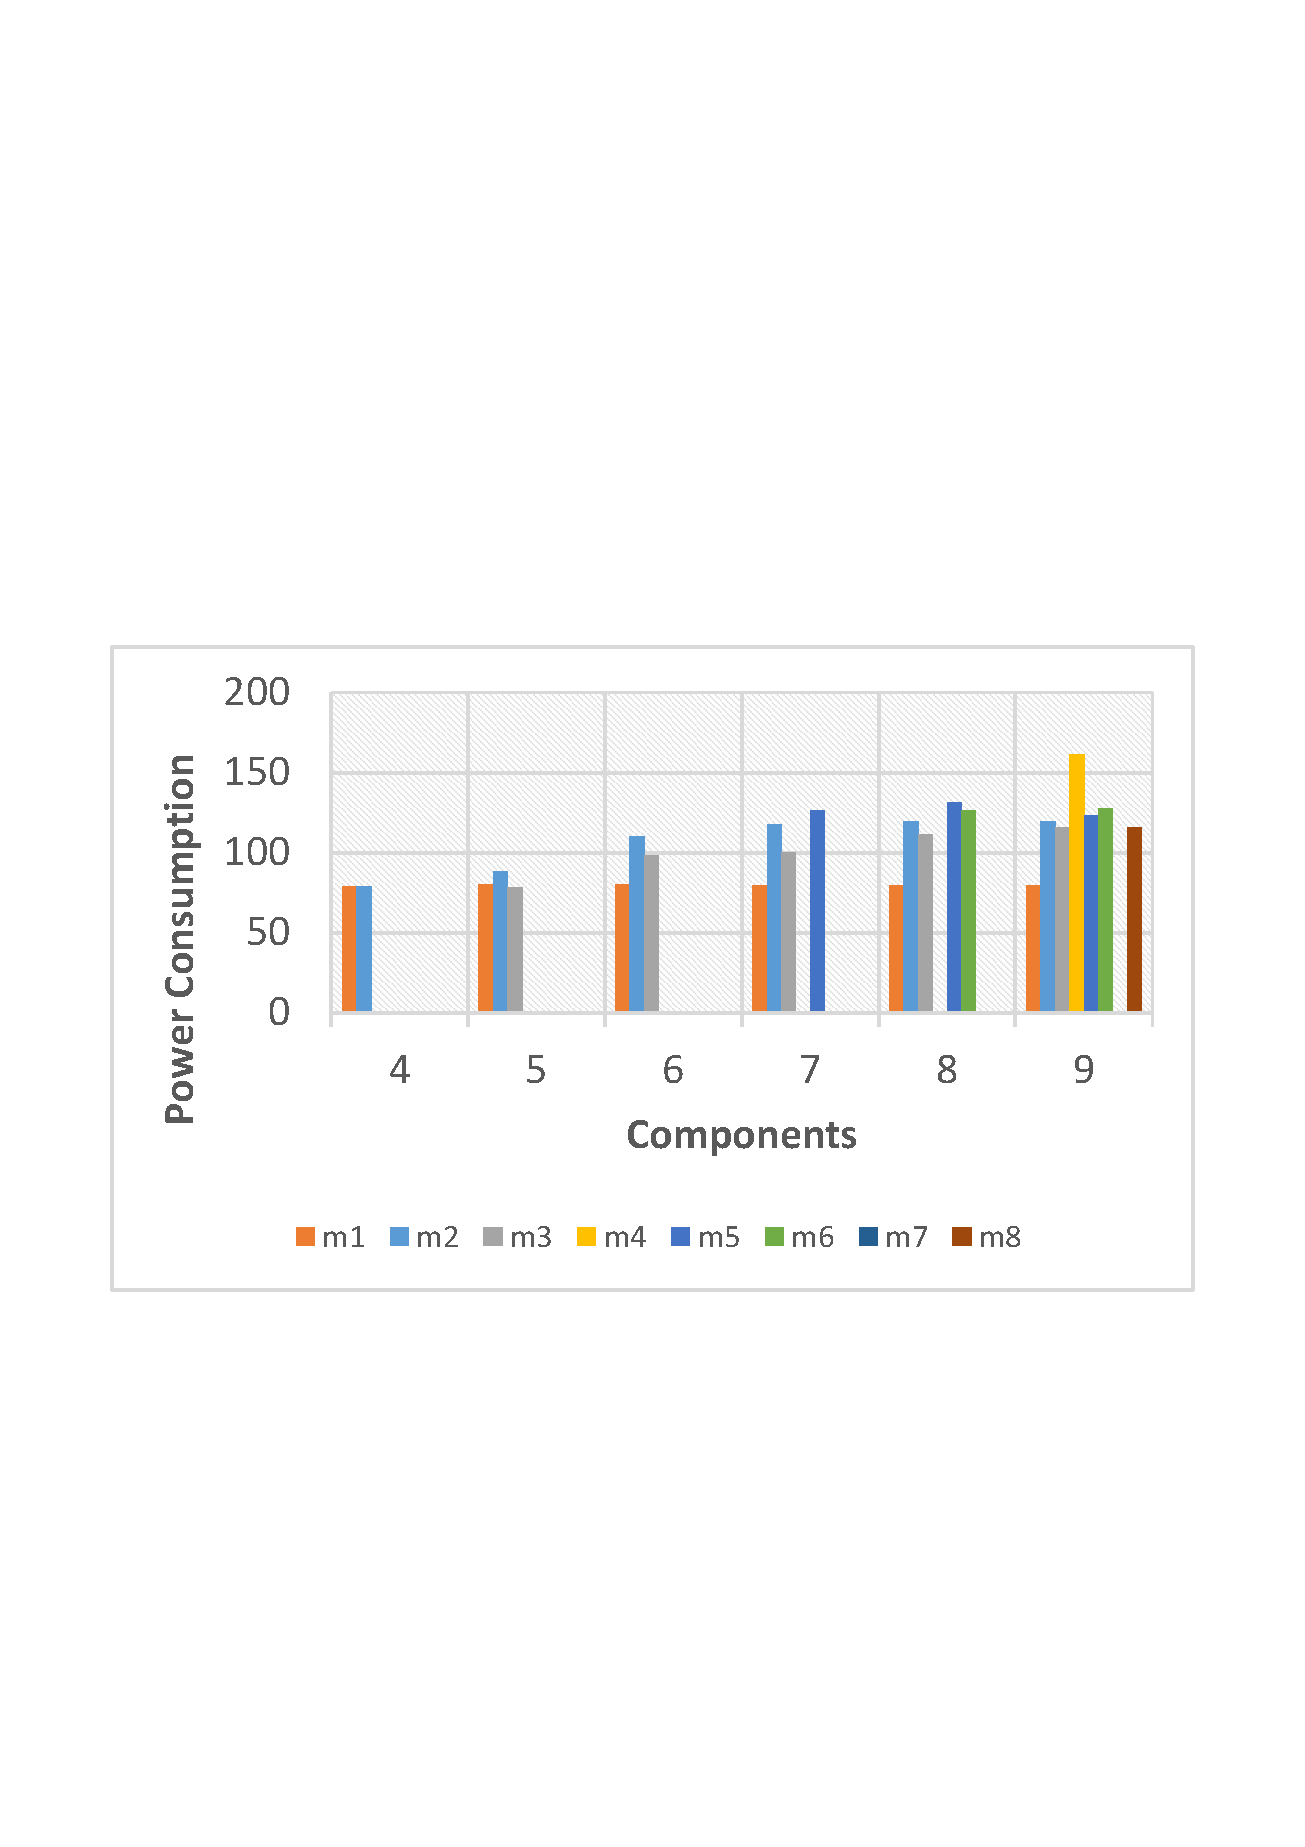
\includegraphics[width=0.45\textwidth]{images/power}
	} ~
	\subfloat[Allocation times software applications.\label{fig_computationtime_ilp}]{% 
		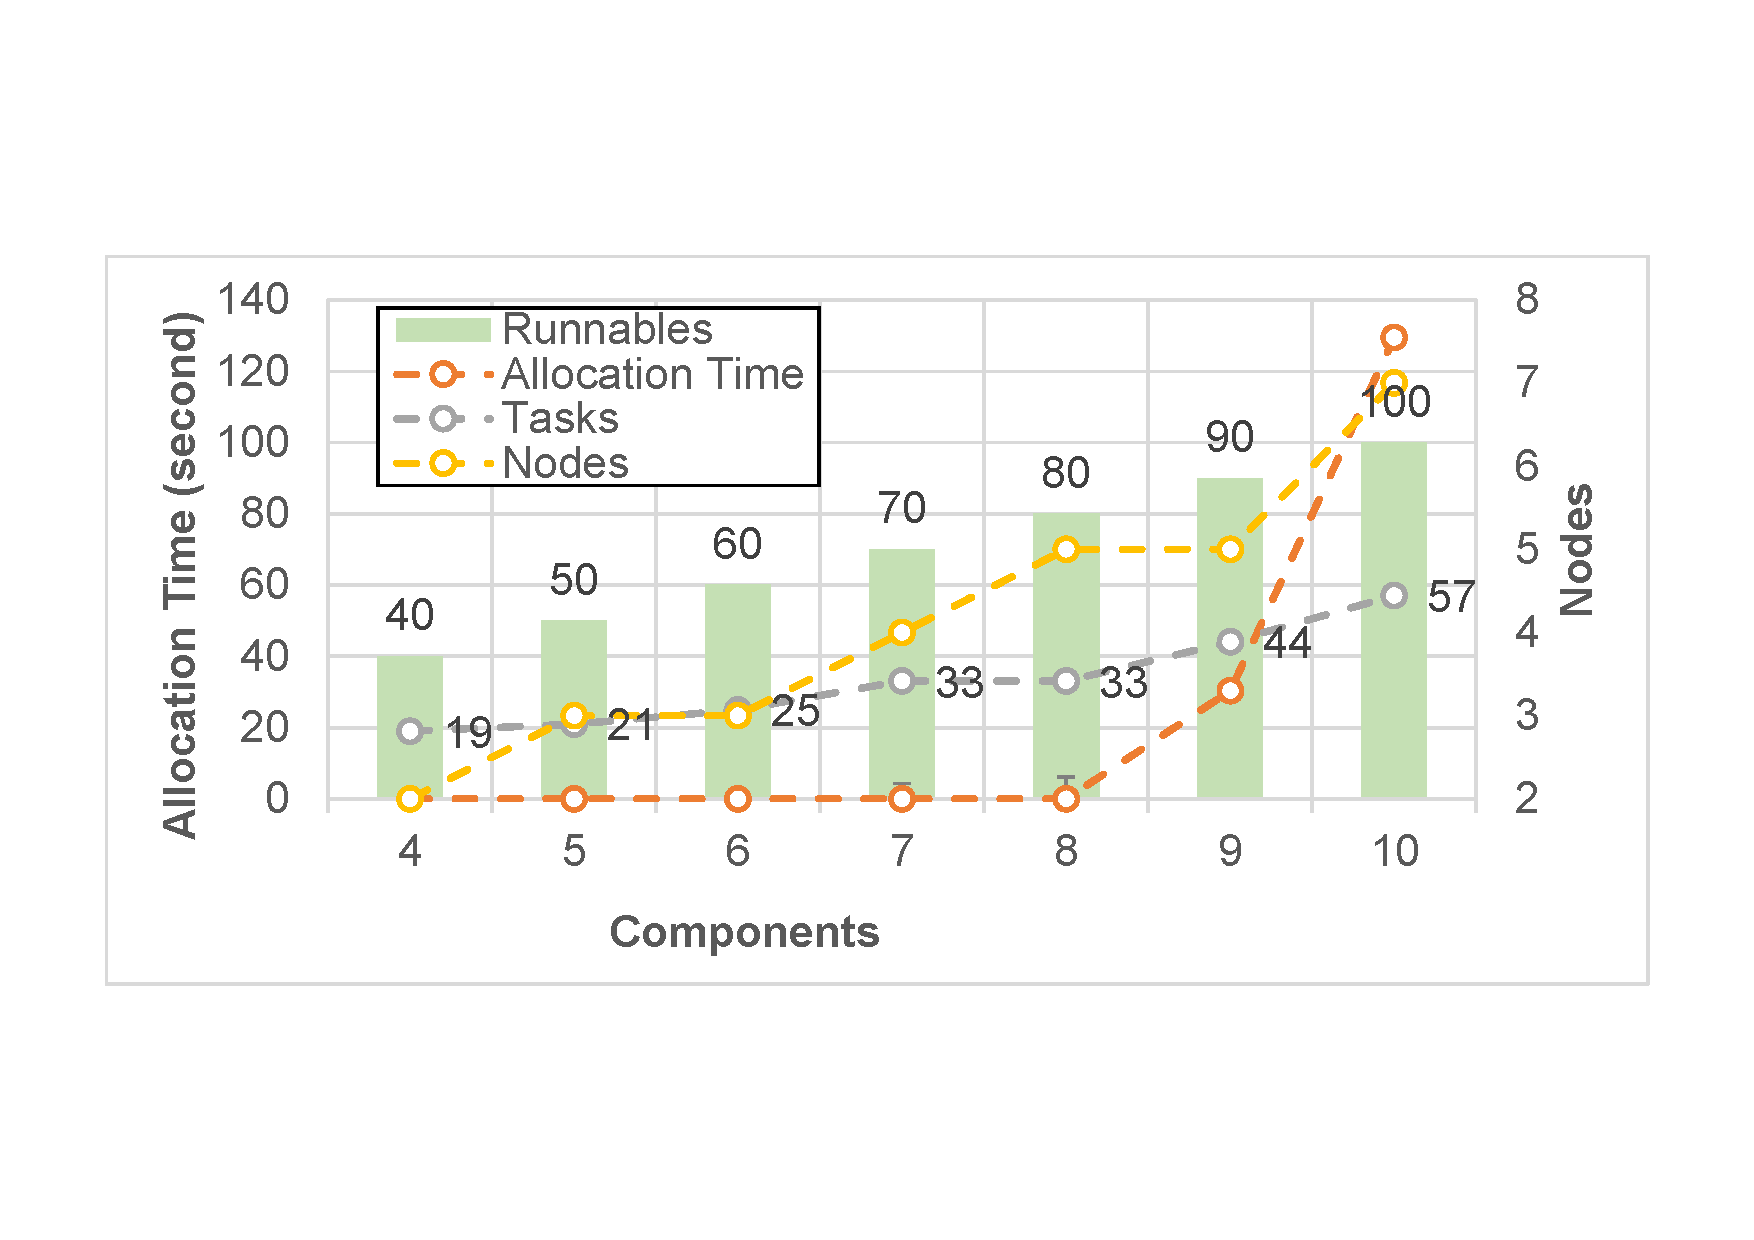
\includegraphics[width=0.55\textwidth]{images/increasing_components} 
	} 
	\caption{ILP optimization of different sizes of software applications based on the number of software components, cause-effect chains, computing nodes.} \label{fig_ilp_results}
\end{figure}

\section{Contr.~5: Metaheuristics-based Software Allocation}\label{rc_pso}
In the previous contribution, we observe that the ILP approach does not scale well to the large software allocation problems. To address this problem, in this section, we propose approximation algorithms based on metahuristics, which is ``high-level problem-independent algorithmic framework that provides a set of guidelines or strategies to develop heuristic optimization algorithms''. Meta-heuristic algorithms does not guarantee optimality of solutions, nevertheless, the solutions can be deemed satisfactory. In the case of minimizing power consumption, what is more appealing to system designers is usually the benefit attained as a result of the power consumption reduction, e.g., accommodating more and more software applications, improving battery-life, rather than optimality. In this spirit, metahuristics can be useful to solve complex and large optimization problems, yet in reasonable time, as compared to exact methods, e.g., branch-and-bound, dynamic programming.

\subsection*{Hybrid Particle-swarm Optimization}
The canonical \pso{} technique uses the constriction factors to balance exploitation and exploration of the search space to get closer to the global optima, hence improving solution quality. Nevertheless, it still suffers from premature convergence or local minima especially when applied on complex and large problems~\cite{Rini2011ParticleChallenges}. Its hybridization is proven to perform better in many cases~\cite{Sengupta2018ParticlePerspectives}. In particular, it is shown to perform better in the tasks assignment problem, that is when hybridized with, e.g., the genetic algorithm~\cite{Sailer2013OptimizingAUTOSAR}, the hill-climbing~\cite{yin2007task}, simulated annealing~\cite{Zhao2007ASystem}, differential evolution~\cite{Storn1997DifferentialSpaces}. As compared to the hybridization with genetic, the hybridization with hill-climbing \hcpso{} is shown to perform better by Yin et al.~\cite{yin2007task} for the tasks allocation problem to maximize reliability of distributed systems. 

In this work, we apply \hcpso{} to the problem at hand, and to tackle its stagnation when applied to large problems. Moreover, we hybridize \pso{} with the differential evolution technique, \depso{}, to improve diversification by applying the mutation and cross-over operators of the differential evolution. Algorithm~\ref{alg_depso} show the pseudocode of the hybrid \pso{}. Line 3 and 4 compute the personal best and the swarm best solutions, respectively. For each particle in the swarm, the velocity and position is computed in Lines~5-8. Lines~9-13 apply the hybridization based on the choice of the algorithm, i.e., \de, \hcpso{} and \shpso{} intermittently, i.e., whenever the interval criterion condition is met.
\IncMargin{1em}
\begin{algorithm}[H]
	\SetAlgoLined
	\SetKwData{P}{P}\SetKwData{S}{sBest}
	\SetKwData{Generation}{Generation}
	\SetKwData{Interval}{Interval}
	\SetKwData{Particles}{Particles}
	\SetKwInOut{Input}{input}\SetKwInOut{Output}{output}
	\SetKwFunction{OptimizeUsingDE}{optimizeUsingDE}
	\SetKwFunction{OptimizeUsingHC}{optimizeUsingHC}
	\SetKwFunction{OptimizeUsingSHC}{optimizeUsingSHC}
	\SetKwFunction{ComputeParticleVelocity}{computeParticleVelocity}
	\SetKwFunction{ComputeParticlePosition}{computeParticlePosition}
	\SetKwFunction{InitPSO}{initPSO}
	\SetKwFunction{ComputePersonalBest}{ComputePersonalBest}
	\SetKwFunction{ComputeSwarmBest}{ComputeSwarmBest}
	
	\BlankLine
	\Input{\pso parameters, \de parameters}
	\Output{Software allocation solution \S .\textbf{x}}
	\BlankLine
	\Particles $P$ $\leftarrow$ \InitPSO{}\;
	\BlankLine
	\While{termination criteria}{
		$\textbf{p}_{bst}$ $\leftarrow$\ComputePersonalBest{$P$}\;
		$\textbf{z}\leftarrow$\ComputeSwarmBest{$P$}\;
		\BlankLine
		\ForEach{$p\in P$}{
			\ComputeParticleVelocity{$p$} according to Equation (\ref{eqn_pso_velocity})\;
			\ComputeParticlePosition{$p$} according to Equation (\ref{eqn_pso_position})\;
		}
		\If{interval criteria}{
			$P$ $\leftarrow$ \OptimizeUsingDE{$P$}\;
			\tcp{$P$ $\leftarrow$ \OptimizeUsingHC{$P$}}\label{hc}
			\tcp{$P$ $\leftarrow$ \OptimizeUsingSHC{$P$}}\label{sh}
		}
	}
	\caption{Hybrid \pso{} Pseudocode.}
	\label{alg_depso}
\end{algorithm}\DecMargin{1em}

\subsection*{Validation on the Bosch EMS Benchmark} 
In this section, we evaluate our proposed hybrid \pso{} algorithms for the allocation of software applications to heterogeneous computing units. The algorithms are evaluated against different specifications of automotive software applications and execution platforms with regard to effectiveness, stability and scalability. The software-application specifications consist of the number of software components $c$, runnables $r$, tasks $t$ and cause-effect chains $g$.  The specifications are synthesized from the automotive benchmark proposed by Kramel et al.~\cite{Kramer2015RealFree}. The benchmark indicates a strong correlation between runnables and cause-effect chains in terms of timing and activation patterns. It shows the timing specifications of runnables and their shares in an engine management system. Moreover, it shows the activation patterns of cause-effect chains, the runnables per activation and their shares in the system. The engine management system is one of the most complex automotive systems in the vehicular electrical/electronic execution platform. 

\noindent\\ \textbf{Result:} We conducted two experiments: i) the first experiment compares the algorithms in terms of quality of solutions, computational time, stability; ii) the second experiment evaluates the effect of applying the approximation algorithm on the overhead of the end-to-end delays calculations due to the replication overhead.

In the first experiment, as illustrated in Figure~\ref{fig_powerconsumption_ilp_metaheuristic}, we show that \ilp returned optimal solutions in the first three problems, likewise all except \pso{} and \depso{}. However, as the problem size increases, the hybrid PSO with the local search algorithms delivered better solutions as compared to \depso{}. 
\begin{figure}
	\centering
	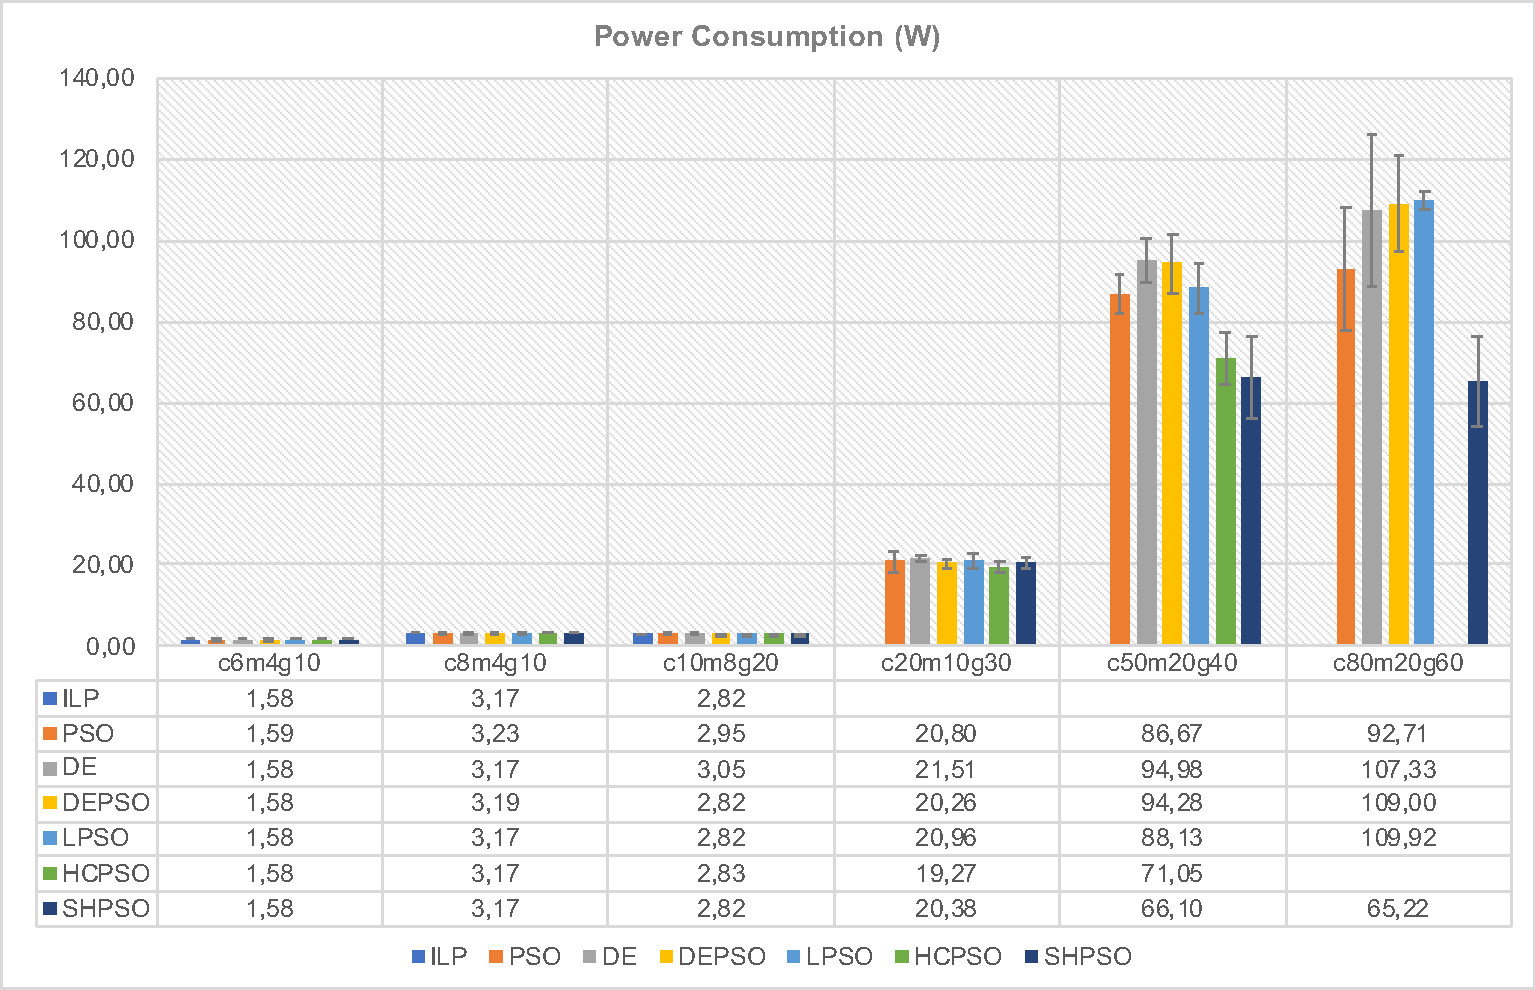
\includegraphics[width=0.8\linewidth]{images/power_consumption.pdf}
	\caption{(Near) Optimal Power Consumption of the Different Software Allocation Problems.}
	\label{fig_powerconsumption_ilp_metaheuristic}\vspace{-0.4cm}
\end{figure}
Futher, we showed that \shpso{} scalled better than \hcpso{} and its results computation time became exponential as shown in Figure~\ref{fig_allocationtime_ilp_metaheuristic} and did not return solutions. In contrast, the hill-climbing-\pso{} hybrid performed the best in all last three problems except \hcpso{} failed to return near optimal solutions to the largest problem \pb{80}{20}{60}. The result also shows that the stochastic version of the hill-climbing-PSO hybrid \shpso{} scales better the over quality of the solution can deemed acceptable as compared to the \ilp{} in the first three problems and \hcpso{} in the next two problems. 
\begin{figure}[h]
	\centering
	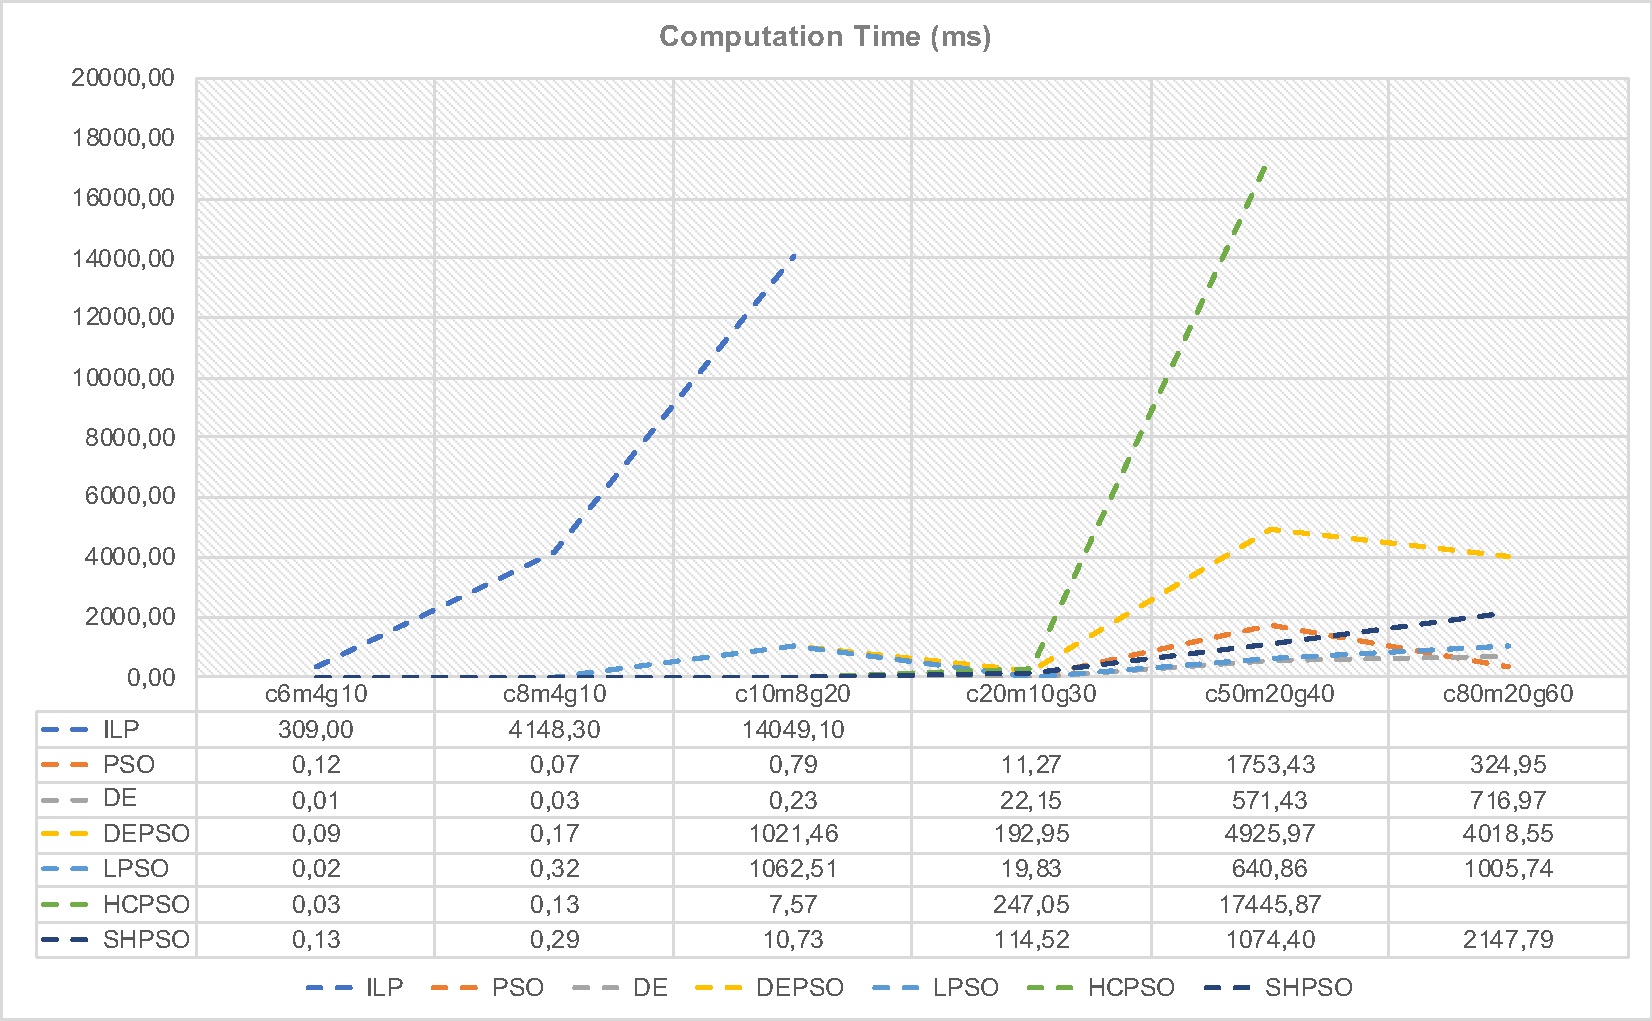
\includegraphics[width=0.8\linewidth]{images/time_summary.pdf}
	\caption{Computation time of the various algorithms for solving different instances of the software allocation problem.}
	\label{fig_allocationtime_ilp_metaheuristic}\vspace{-0.4cm}
\end{figure}

Due to the replication of components to meet the reliability goals, the overhead of computing the delays is exponential. Figure~\ref{fig_chainsreplicationimprovements} compares the effect of with and without applying the approximation algorithm.  It shows that $61\%-81\%$ computational time improvement over the exact method while facing quality degradation only for samples $g_{30}d_{3}$ and  $g_{60}d_{2}$. The improvements are in seconds, which means for a single usage (or run) of the meta-heuristic optimization algorithms, it is not significant. However, considering practical engineering process, which requires several iterations, the commutative effect of appliying the approaximation algorithm can beneficial in terms of responsiveness to engineers. 
\begin{figure}[h]
	\centering
	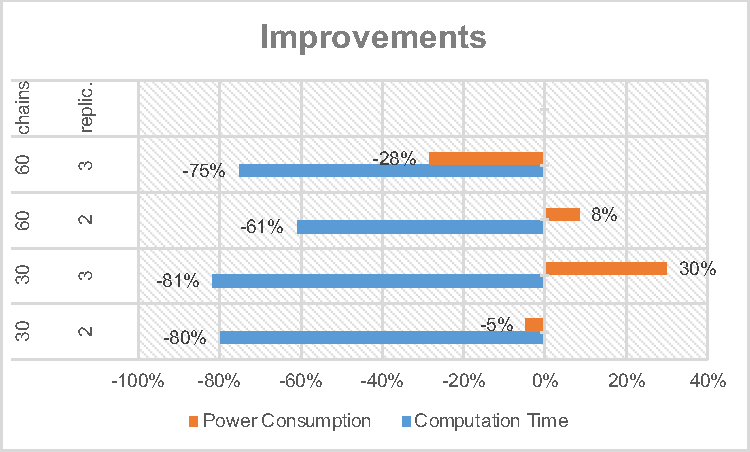
\includegraphics[width=0.7\linewidth]{images/chains_replication_improvements}
	\caption{Effect of approximate algorithm over delay calculations with replication.}
	\label{fig_chainsreplicationimprovements}
\end{figure}

\section{Paper Contributions}
Tables~\ref{paper_contribution} shows the peer-reviewed papers and their contribution to the thesis.
% Please add the following required packages to your document preamble:
% \usepackage{booktabs}
\begin{table}[h]
	\begin{tabular}{@{}llllll@{}}
		\toprule
		Paper & Sec\ref{rc_resa} & Sec\ref{rc_resaanalysis}& Sec\ref{rc_sim} & Sec\ref{rc_ilp} & Sec\ref{rc_pso}\\ \midrule
		A & $\times$ &  &  &  &\\
		B & $\times$ & $\times$ &  & & \\
		C &  & $\times$ &  & & \\
		D &  &  & $\times$ &  &\\
		E &  &  &  & $\times$ &\\
		F &  &  &  & $\times$ &$\times$ \\ \bottomrule
	\end{tabular}
\caption{List of the peer-reviewed papers and their contribution to the thesis.}\label{paper_contribution}
\end{table}
\subsection*{Paper A}
ReSA: An ontology-based requirement specification language tailored to automotive systems. Nesredin~Mahmud, Cristina~Seceleanu and Oscar~Ljungkrantz.\textit{In the 10th IEEE International Symposium on Industrial Embedded Systems (SIES)(pp. 1-10). IEEE, 2015}.\label{lbl_resa}\\[6pt]
\textbf{Abstract:} \textit{Automotive systems are developed using multi-leveled architectural abstractions in an attempt to manage the increasing complexity and criticality of automotive functions. Consequently, well-structured and unambiguously specified requirements are needed on all levels of abstraction, in order to enable early detection of possible design errors. However, automotive industry often relies on requirements specified in ambiguous natural language, sometimes in large and incomprehensible documents. Semi-formal requirements specification approaches (e.g., requirement boilerplates, pattern-based specifications, etc.) aim to reduce requirements ambiguity, without altering their readability and expressiveness. Nevertheless, such approaches do not offer support for specifying requirements in terms of multi-leveled architectural concepts, nor do they provide means for early-stage rigorous analysis of the specified requirements. In this paper, we propose a language, called ReSA, which allows requirements specification at various levels of abstraction, modeled in the architectural language of EAST-ADL. ReSA uses an automotive systems' ontology that offers typing and syntactic axioms for the specification. Besides enforcing structure and more rigor in specifying requirements, our approach enables checking refinement as well as consistency of requirements, by proving ordinary boolean implications. To illustrate ReSA's applicability, we show how to specify some requirements of the Adjustable Speed Limiter, which is a complex, safety-critical Volvo Trucks user function.}\\[6pt]
\textbf{Personal Contributions: }I was the main driver of the paper. I developed the ReSA language including its syntax and semantics, and Cristina Seceleanu proposed a consistency analysis technique besides giving useful comments and ideas on the design of the language. Oscar Ljungkrantz provided useful materials from VGTT that were eventually analyzed for the language development, and gave feedback on the language design and implementation from an industrial viewpoint.\\
\textbf{Status:} Published

\subsection*{Paper B}
ReSA tool: Structured requirements specification and SAT-based consistency-checking. Nesredin~Mahmud, Cristina~Seceleanu and Oscar~Ljungkrantz. \textit{In the 2016 Federated Conference on Computer Science and Information Systems (FedCSIS)(pp. 1737-1746). IEEE, 2016.}\label{lbl_resatool}\\[6pt]
\textbf{Abstract:} \textit{Most industrial embedded systems requirements are
	specified in natural language, hence they can sometimes be
		ambiguous and error-prone. Moreover, employing an early-stage
		model-based incremental system development using multiple
		levels of abstraction, for instance via architectural languages
		such as EAST-ADL, calls for different granularity requirements
		specifications described with abstraction-specific concepts that
		reflect the respective abstraction level effectively.
		In this paper, we propose a toolchain for structured requirements
		specification in the ReSA language, which scales to multiple
		EAST-ADL levels of abstraction. Furthermore, we introduce
		a consistency function that is seamlessly integrated into the
		specification toolchain, for the automatic analysis of requirements
		logical consistency prior to their temporal logic formalization
		for full formal verification. The consistency check subsumes
		two parts: (i) transforming ReSA requirements specification into
		boolean expressions, and (ii) checking the consistency of the
		resulting boolean expressions by solving the satisfiability of their
		conjunction with the Z3 SMT solver. For validation, we apply
		the ReSA toolchain on an industrial vehicle speed control system,
		namely the Adjustable Speed Limiter.}\\[6pt]%abstract
	\textbf{Personal Contributions: }I was the main driver of the paper. I developed the ReSA toolchain that consists of the editor and the consistency checker including the integration with the Z3 SAT solver in the backend. Cristina Seceleanu formulated the consistency checking and together with Oscar Ljungkrantz, they contributed to the paper with useful comments and ideas.\\
		\textbf{Status: }Published

\subsection*{Paper C}
	Specification and semantic analysis of embedded systems requirements: From description logic to temporal logic. Nesredin~Mahmud, Cristina~Seceleanu and Oscar~Ljungkrantz. \textit{In the International Conference on Software Engineering and Formal Methods (SEFM)(pp. 332-348). Springer, Cham, 2017.}\label{lbl_resadl}\\[6pt]%authors
	\textbf{Abstract:} \textit{Due to the increasing complexity of embedded systems, early detection of software/hardware errors has become desirable. In this context, effective yet flexible specification methods that support rigorous analysis of embedded systems requirements are needed. Current specification methods such as pattern-based, boilerplates normally lack meta-models for extensibility and flexibility. In contrast, formal specification languages, like temporal logic, Z, etc., enable rigorous analysis, however, they usually are too mathematical and difficult to comprehend by average software engineers. In this paper, we propose a specification representation of requirements, which considers thematic roles and domain knowledge, enabling deep semantic analysis. The specification is complemented by our constrained natural language specification framework, ReSA, which acts as the interface to the representation. The representation that we propose is encoded in description logic, which is a decidable and computationally-tractable ontology language. By employing the ontology reasoner, Hermit, we check for consistency and completeness of requirements. Moreover, we propose an automatic transformation of the ontology-based specifications into Timed Computation Tree Logic formulas, to be used further in model checking embedded systems.}\\[6pt]%abstract
	\textbf{Personal Contributions:} I was the main driver of the language. I developed the ReSA language semantics using event-base approach, which is encoded in description logic. Cristina~Seceleanu and Ljungkrantz~Oscar provided with useful ideas and comments.\\
	\textbf{Status:} Published

\subsection*{Paper D}
SIMPPAAL - A Framework For Statistical Model Checking of Industrial Simulink Models. Predrag~Filipovikj, Nesredin~Mahmud, Raluca~Marinescu, Cristina~Seceleanu, Oscar~Ljungkrantz and Henrik~L\"{o}nn. \textit{Submitted to ACM Transactions on Software Engineering and Methodology (TOSEM).}\label{lbl_simulink_ilp}
\\[3pt]{\footnotesize This article is an extended version of the following conference paper:
     Simulink to UPPAAL Statistical Model Checker: Analyzing Automotive Industrial Systems.
Predrag Filipovikj, Nesredin Mahmud, Raluca Marinescu, Cristina Seceleanu, Oscar Ljungkrantz, Henrik L{\"o}nn. In Proceedings of the 21st International
Symposium on Formal Methods (FM2016), pages 748-756. Limassol, Cyprus. Springer, LNCS, November 2016. Revisions required. }\\[6pt]%authors
	\noindent \textbf{Abstract:} \textit{The evolution of automotive systems has been rapid. Nowadays, electronic brains control dozens of functions in vehicles, like
		braking, cruising, etc. Model-based design approaches, in environments such as MATLAB Simulink, seem to help in addressing
		the ever-increasing need to enhance quality, and manage complexity, by supporting functional design from a set of block
		libraries, which can be simulated and analyzed for hidden errors, but also used for code generation. For this reason, providing
		assurance that Simulink models fulfill given functional and timing requirements is desirable. In this paper, we propose a
		pattern-based, execution-order preserving automatic transformation of atomic and composite Simulink blocks into stochastic
		timed automata that can then be formally analyzed with Uppaal Statistical Model Checker (Uppaal SMC). To enable this, we
		first define the formal syntax and semantics of Simulink blocks and their composition, and show that the transformation is
		provably correct for a certain class of Simulink models. Our method is supported by the SIMPPAAL tool, which we introduce
		and apply on two industrial Simulink models, a prototype called the Brake-by-Wire and an operational Adjustable Speed
		Limiter system. This work enables the formal analysis of industrial Simulink models, by automatically generating stochastic
		timed automata counterparts.}\\[6pt]%abstract
	\textbf{Personal Contributions: } The three co-authors contributed equally to writing the paper. Technically, I equally contributed with proposing the pattern-based semantics of Simulink blocks, together with Predrag Filipovikj. I introduced a mechanism to enforce the execution order of the blocks using inter-arrival times. Predrag implemented the flattening algorithm and the tool for the automatic transformation of Simulink models into a network of timed automata with stochastic semantics. Raluca Marinescu contributed with analyzing the BBW system, Cristina Seceleanu contributed with defining the methodology, and with useful ideas and comments. Guillermo Rodriguez-Navas wrote the related work section. The industrial coauthors provided the use cases and commented on the final draft.\\
	\noindent\textbf{Status:} Revisions required. 

\subsection*{Paper E}
Power-aware Allocation of Fault-tolerant Multirate AUTOSAR Applications.
     Nesredin~Mahmud, Guillermo~Rodriguez-Navas, Hamid~Faragardi, Saad~Mubeen and Cristina~Seceleanu. \textit{In the 25th Asia-Pacific Software Engineering Conference (APSEC'18). IEEE.}  
     \label{lbl_softwareallocation_ilp}
\\[6pt]%authors
\textbf{Abstract:} \textit{The growing complexity of automotive functionality has attracted revolutionary computing architectures such as mixed-criticality design, which enables effective consolidation of software applications with different criticality on a shared execution platform. Mixed-critical design that is required to satisfy end-to-end timing and reliability specifications should consider power-efficient software design in order to accommodate more and more functionality. Due to the recursive and exhaustive nature of the real-time and reliability analysis, exact methods, e.g., branch and bound, dynamic programming, are prohibitively expensive. We propose hybrid particle-swarm optimization algorithms based on differential evolution and hill-climbing algorithms to minimize power consumption of the safety-critical software, which have end-to-end timing and reliability requirements, on a network of heterogeneous computing units. The optimization approach employs fault tolerance to maximize reliability of the software applications subsequently meet the reliability requirements. Our proposed integrated software-allocation approach is evaluated using a range of synthetic software applications based a real-world automotive benchmark. The evaluation makes comparative analysis of the differential evolution, particle-swarm optimization, integer-linear programming and hybrid particle-swarm optimization algorithms. The results show that the hybrid algorithms based on the hill-climbing algorithms outperform the rest of the meta-heuristic algorithms, in particular, the stochastic version of the hill-climbing algorithm scales well in large software allocation optimization problems while its overall optimality performance can be deemed acceptable.
}\\[6pt]%abstract
\textbf{My Contributions: } I was the main driver of the paper. I developed the system model with the guidance of the co-authors, and formulated the optimization problem with the guidance of Hamid~Faragardi, implemented the the problem in Java, and collected and analyzed the experimental results. The co-authors gave writing updates, useful ideas and comments on the paper, and specifically: Guillermo~Rodriguez-Navas on reliability analysis, Hamid~Faragardi on optimization, Saad~Mubeen on the timing analysis and Cristina~Seceleanu on the objective function and constraints.\\
\textbf{Status:} Published

\subsection*{Paper F}
Optimized Allocation of Fault-tolerant Embedded Software with End-to-end Timing Constraints.	\textit{M\"{a}lardalen Real-time Research Center Technical Report (MRTC), ISRN MDH-MRTC-325/2019-1-SE, 2019}. Submitted to Elsevier Journal of Systems Architecture (JSA).\\[6pt]%authors
\textbf{Abstract:} \textit{It is desirable to optimize power consumption of distributed safety-critical software that realize fault tolerance and maximize reliability as a result, to support the increasing complexity of software functionality in safety-critical embedded systems. Likewise, safety-critical applications that are required to meet end-to-end timing constraints may require additional computing resources. In this paper, we propose a scalable software-to-hardware allocation based on hybrid particle-swarm optimization with hill-climbing and differential algorithms to efficiently map software components to a network of heterogeneous computing nodes while meeting the timing and reliability constraints. The approach assumes fixed-priority preemptive scheduling, and delay analysis that value freshness of data, which is typical in control software applications.
Our proposed solution is evaluated on a range of software applications, which are synthesized from a real-world automotive AUTOSAR benchmark. The evaluation makes comparative analysis of the different algorithms, and a solution based on integer-linear programming, which is an exact method. The results show that the hybrid with the hill-climbing algorithms return very close solutions to the exact method and outperformed the hybrid with the differential algorithm, though consumes more time. The hybrid with the stochastic hill-climbing algorithm scales better and its optimality can be deemed acceptable.}\\[6pt]%abstract
\textbf{Personal Contributions: } I was the main driver of the paper. I developed the system model with the guidance of the co-authors, and formulated the optimization problem with the guidance of Hamid~Faragardi, implemented the the problem in Java, and collected and analyzed the experimental results. The co-authors gave writing updates, useful ideas and comments on the paper, and specifically: Guillermo~Rodriguez-Navas on reliability analysis, Hamid~Faragardi on optimization, Saad~Mubeen on the timing analysis and Cristina~Seceleanu on the objective function and constraints. \\%my contribution
\textbf{Status:} Submitted to Journal of System Architecture (JSA), Elsevier Journals.\\
